\documentclass[11pt]{article}

\usepackage[T1]{fontenc}
\usepackage[utf8]{inputenc}
\usepackage{lmodern}
\usepackage{microtype}
\usepackage[a4paper,margin=25mm]{geometry}
\usepackage{amsmath,amssymb,amsthm,mathtools}
\usepackage{booktabs,longtable,tabularx,array}
\usepackage{enumitem}
\usepackage[numbers,sort&compress]{natbib}
\usepackage{xcolor}
\usepackage{tikz}
\usetikzlibrary{positioning,arrows.meta}
\usepackage{hyperref}
\usepackage[nameinlink,capitalize,noabbrev]{cleveref}
\usepackage{seqsplit}
\usepackage{listings}
\usepackage{caption}

\hypersetup{
  pdftitle={Conditioning on the Largest Color Classes: Certified Bounds for Minimum-Sum Coloring of Very Dense Benchmark Graphs},
  pdfauthor={Olawale Titiloye},
  colorlinks=true,
  linkcolor=blue!45!black,
  citecolor=blue!45!black,
  urlcolor=blue!45!black
}
\setlist{nosep,leftmargin=2em}
\setlength{\parindent}{1.2em}
\setlength{\parskip}{0.15em}
\setlength{\tabcolsep}{5pt}
\emergencystretch=3em

\newtheorem{theorem}{Theorem}[section]
\newtheorem{lemma}[theorem]{Lemma}
\newtheorem{proposition}[theorem]{Proposition}
\newtheorem{corollary}[theorem]{Corollary}
\theoremstyle{definition}
\newtheorem{definition}[theorem]{Definition}
\newtheorem{remark}[theorem]{Remark}

\newcommand{\DSJCTwoFifty}{\textnormal{\textsc{DSJC250.9}}}
\newcommand{\DSJCFiveHundred}{\textnormal{\textsc{DSJC500.9}}}
\newcommand{\DSJCThousand}{\textnormal{\textsc{DSJC1000.9}}}
\newcommand{\CTwoThousand}{\textnormal{\textsc{C2000.9}}}
\newcommand{\Stable}{\mathcal{S}}
\newcommand{\Res}{\mathcal{Q}}
\newcommand{\odd}{\operatorname{odd}}
\newcommand{\hashvalue}[1]{\begingroup\ttfamily\scriptsize\seqsplit{#1}\endgroup}
\newcolumntype{Y}{>{\raggedright\arraybackslash}X}

\lstdefinestyle{paperlisting}{
  basicstyle=\ttfamily\footnotesize,
  columns=fullflexible,
  frame=single,
  breaklines=true,
  showstringspaces=false,
  xleftmargin=0.5em,
  xrightmargin=0.5em
}
\title{Conditioning on the Largest Color Classes:\\
Certified Bounds for Minimum-Sum Coloring of Very Dense Benchmark Graphs}
\author{Olawale Titiloye}
\date{24 September 2026}

\begin{document}
\maketitle

\begin{abstract}
In the minimum-sum coloring problem the cost of a coloring after canonical
relabeling depends only on the sizes of its color classes, so lower bounds
can be obtained by optimizing over class-size profiles. Such bounds do not
see whether stable sets of the
required sizes can coexist. We strengthen them by conditioning on which
maximum stable sets are color classes and then bounding, layer by layer, the
stable sets that can still be packed into the remaining vertices. Each bound
is certified by exact rational dual inequalities, combined where necessary by
exhaustive branching, over stable-set families enumerated completely from the
graph.

For the DIMACS graph \DSJCTwoFifty{} this proves that the chromatic sum is
$8{,}277$, the value of colorings reported in the literature; the lower bound
previously reported was $7{,}882$. We also prove
$29{,}791\le\Sigma(\DSJCFiveHundred)\le29{,}848$ and
$102{,}344\le\Sigma(\DSJCThousand)\le103{,}256$, raising the previously
reported lower bounds of $29{,}768$ and $100{,}078$, and
$381{,}823\le\Sigma(\CTwoThousand)\le382{,}379$. For \CTwoThousand{} the lower
bound coincides with the optimum of the stable-set linear relaxation, and for
\DSJCFiveHundred{} the three lowest remaining cases admit fractional
solutions of the conditioned relaxation, so raising either lower bound requires
arguments beyond that relaxation. All four graphs have independence number 5
or 6, which is what makes the complete enumerations possible.
\end{abstract}

\section{Introduction}
\label{sec:introduction}

In the minimum-sum coloring problem (MSCP), introduced by Kubicka and
Schwenk~\cite{kubicka1989}, the vertices of a graph receive positive integer
colors, adjacent vertices receive different colors, and the sum of the colors
is to be minimized. The minimum is the \emph{chromatic sum} $\Sigma(G)$.
Every vertex pays the label of its class, so in an optimal coloring larger
classes receive smaller labels, and the cost is determined by the sorted
sizes of the classes. The number of colors enters only through those sizes:
a coloring with more than $\chi(G)$ colors can have a smaller sum, because
the gain from a large class at a small label can outweigh the cost of an
extra small class at the end.

Lower bounds for the problem have developed along two lines. The first
discards part of the graph's structure. A partition of the vertices into
cliques gives a bound, since a clique of size $k$ needs $k$ distinct
labels~\cite{moukrim2010,wuhao2013}; it keeps the incompatibilities inside
each clique and discards the edges between cliques. Profile relaxations go
further and keep only the sizes of the classes, constrained by a few graph
invariants. Lecat, Lucet and
Li~\cite{lecat2017} minimize the sorted-profile cost over integer partitions
of~$n$ whose parts are at most $\alpha(G)$ and whose number of parts is at
least a lower bound on $\chi(G)$. Gondran, Duchamp and Moalic~\cite{gondran2019}
add a cap on the number of parts equal to $\alpha(G)$, computed from the
intersection graph of the maximum stable sets; without the cap, their
relaxation reduces to that of Lecat et al. The second line keeps the graph
intact through stable-set formulations, in which a variable selects each
possible color class. Mehrotra and Trick~\cite{mehrotra1996} showed how to
solve this formulation of ordinary coloring by column generation. It has been
adapted to MSCP by Furini et al.~\cite{furini2018} and Mrad et
al.~\cite{mrad2020}, and used in a branch-and-price algorithm by Delle Donne
et al.~\cite{delledonne2021}. Tammal and A\"ider~\cite{tammal2025} give an
exact method based instead on modular decomposition.

What profile relaxations cannot see is simultaneous compatibility. A profile
may ask for many large classes even though every choice of those classes
leaves too little room for the smaller ones. The cap of Gondran et al.
records how many maximum classes can coexist, but not what a particular
choice of them leaves behind, and two maximum stable sets of the same size
can leave very different room below them; \cref{fig:five-vertex} shows the
smallest kind of example. This paper conditions on the identities of the
largest color classes and then bounds, one layer at a time, how many stable
sets of each smaller size can still be packed. The bounds are certified by
exact rational dual inequalities, combined, when one inequality is not
enough, into trees of inequalities obtained by exhaustive branching. They are
checked against families of stable sets enumerated completely from the graph.

Complete enumeration is possible because the graphs we study are very dense.
Held, Cook and Sewell~\cite{held2012} note that in graphs of edge density
about $0.9$ the maximal stable sets are few and small enough to enumerate;
their safe branch-and-price settled the chromatic number of \DSJCTwoFifty{},
which is $72$~\cite[Table~3]{held2012}. We work with four DIMACS graphs of
this density, \DSJCTwoFifty{}, \DSJCFiveHundred{}, \DSJCThousand{} and
\CTwoThousand{}, whose independence numbers are 5 or~6.

\subsection{Results}

\begin{theorem}
\label{thm:main-intro}
The chromatic sums of the four benchmark graphs\footnote{The graph files, and
the identities that bind the theorem to them, are specified in
\cref{app:files}.} satisfy
\begin{enumerate}[label=(\roman*)]
  \item $\Sigma(\DSJCTwoFifty)=8{,}277$;
  \item $29{,}791\le\Sigma(\DSJCFiveHundred)\le29{,}848$;
  \item $102{,}344\le\Sigma(\DSJCThousand)\le103{,}256$;
  \item $381{,}823\le\Sigma(\CTwoThousand)\le382{,}379$.
\end{enumerate}
\end{theorem}

Every upper bound comes from an explicit coloring checked against the graph.
The colorings were found by the author's coloring searches, followed for
\CTwoThousand{} by the reoptimization described in \cref{sec:c2000}. Since
each is checked directly, the bounds do not depend on how the colorings were
found. \Cref{tab:results} compares the bounds with those reported in the
literature.

\begin{table}[t]
\centering
\small
\caption{Bounds for the four graphs. The reported values are taken from the
tables cited in the notes; their proofs and colorings were not replayed here.
The bounds of this paper are proved in the sections indicated, and the gap is
the difference between them.}
\label{tab:results}
\begin{tabular}{@{}lrrrrrrrl@{}}
\toprule
& & & \multicolumn{2}{c}{reported} & \multicolumn{3}{c}{this paper} & \\
\cmidrule(lr){4-5}\cmidrule(lr){6-8}
graph & $n$ & $\alpha$ & lower & upper & lower & upper & gap & section\\
\midrule
\DSJCTwoFifty{}    & 250   & 5 & $7{,}882^{a}$   & $8{,}277^{b}$   & $8{,}277$   & $8{,}277$   & $0$   & \ref{sec:dsjc250}\\
\DSJCFiveHundred{} & 500   & 5 & $29{,}768^{a}$  & $29{,}856^{c}$  & $29{,}791$  & $29{,}848$  & $57$  & \ref{sec:dsjc500}\\
\DSJCThousand{}    & 1,000 & 6 & $100{,}078^{a}$ & $103{,}429^{c}$ & $102{,}344$ & $103{,}256$ & $912$ & \ref{sec:dsjc1000}\\
\CTwoThousand{}    & 2,000 & 6 & ---$^{d}$       & ---$^{d}$       & $381{,}823$ & $382{,}379$ & $556$ & \ref{sec:c2000}\\
\bottomrule
\end{tabular}

\smallskip
\begin{minipage}{0.94\textwidth}
\footnotesize
$^{a}$~Gondran et al.~\cite[Table~1]{gondran2019} (preprint).
$^{b}$~Lecat et al.~\cite[Table~2]{lecat2017}; also reported
in~\cite{moukrim2013,jinhao2016}.
$^{c}$~EBES~\cite[Table~1]{wuetal2018}, five-hour runs.
$^{d}$~No MSCP values were located in the principal heuristic tables
of~\cite{wuhao2012,moukrim2013,jinhao2016,wuetal2018}.
\end{minipage}
\end{table}

For \DSJCTwoFifty{} the reported lower bounds rose from $4{,}179$ by clique
decomposition~\cite[Table~1]{wuhao2013} to $6{,}651$ with
motifs~\cite[Table~2]{lecat2017} and $7{,}882$ with the cap on maximum
classes~\cite[Table~1]{gondran2019}, while colorings of sum $8{,}277$ were
reported in~\cite{moukrim2013,jinhao2016,lecat2017}; the EXSCOL heuristic
reported $8{,}286$~\cite[Table~1]{wuhao2012}. \Cref{thm:main-intro}(i) closes
this gap. For \DSJCFiveHundred{} and \DSJCThousand{} our lower bounds exceed
those reported by Gondran et al.\ by $23$ and $2{,}266$, and our colorings
improve the EBES values by $8$ and $173$. Of the $2{,}266$ gained on
\DSJCThousand{}, a feasible dual of the unconditioned stable-set relaxation
already accounts for $2{,}231$, since its value rounds up to $102{,}309$;
conditioning on the three stable 6-sets adds the remaining $35$
(\cref{sec:dsjc1000}). For \CTwoThousand{} the lower bound is the profile
bound of Gondran et al.\ evaluated with a certified cap, and the stable-set
relaxation attains it exactly (\cref{sec:c2000}).

\subsection{What is inherited and what is new}

Several ingredients come from earlier work. The partition relaxations that
work with sorted class sizes are those of Lecat et al.~\cite{lecat2017} and
Gondran et al.~\cite{gondran2019}. We
write profiles in Ferrers (conjugate-partition)
coordinates~\cite{andrews1998}, which also appear in integer-programming
formulations~\cite{gavenciak2019}, because in these coordinates the objective
becomes a sum of triangular numbers. The cap on the number of maximum classes
is that of Gondran et al.; we compute its value exactly and certify it. The
stable-set master of \cref{sec:master} is a stable-set formulation in the
tradition of Mehrotra and Trick, with the sum objective written in Ferrers
coordinates. Our lower bounds
rest, like the safe bounds of Held, Cook and Sewell~\cite{held2012}, on dual
solutions with integer data whose feasibility is verified exactly, and our
branch trees are checked in the spirit of certified
branch-and-bound~\cite{larrosa2011,cheung2017}.

The contribution of this paper is the conditioning and its certification:
fixing the identities of the top classes, bounding the layers below them by
lexicographic scores, and certifying each bound by exact dual inequalities
and exhaustively branched trees over complete residual stable-set families
(\cref{sec:conditioning}). With these tools we prove the bounds of
\cref{thm:main-intro}. The same analysis locates where the approach stops.
The three lowest open cases for \DSJCFiveHundred{} admit fractional solutions
of the conditioned relaxation (\cref{sec:dsjc500-limits}), and for
\CTwoThousand{} the profile bound already equals the optimum of the
stable-set relaxation (\cref{sec:c2000}).

\subsection{Organization}

\Cref{sec:profiles} develops profiles, Ferrers coordinates and the stable-set
master. \Cref{sec:conditioning} introduces top packings and envelopes and the
certificates that bound them. \Cref{sec:dsjc250} proves
$\Sigma(\DSJCTwoFifty)=8{,}277$, \cref{sec:dsjc500} proves the bound for
\DSJCFiveHundred{} and shows why its three lowest cases resist, and
\cref{sec:larger} conditions the stable-set relaxation for \DSJCThousand{} and
evaluates it for \CTwoThousand{}. \Cref{sec:verification} explains how the
results are checked, and \cref{sec:conclusion} discusses what the method
needs and what remains open. The appendices hold the proof data for
\DSJCTwoFifty{} (\cref{app:dsjc250-data,app:witnesses}), two supplementary
analyses that no proof depends on (\cref{app:splitting,app:neighbourhood}),
the file identities and replay commands (\cref{app:files}), and a table of
notation (\cref{app:notation}).

\section{Profiles and the stable-set master}
\label{sec:profiles}

\subsection{Class-size profiles and Ferrers coordinates}

Let $G=(V,E)$ be a finite simple graph with $n=|V|$. A proper sum coloring is a
map $c:V\to\mathbb{Z}_{>0}$ with $c(u)\ne c(v)$ for every $uv\in E$; its value
is $\sum_{v\in V}c(v)$, and $\Sigma(G)$ is the least value of a proper sum
coloring. The nonempty color classes are stable sets. Deleting unused labels
and compressing the others to $1,\ldots,\ell$ cannot increase the sum, so we
write the classes as $C_1,\ldots,C_\ell$, with the subscript as color.

For a fixed partition into stable classes, consecutive labels should be
assigned in nonincreasing order of class size: if $i<j$ but $|C_i|<|C_j|$,
exchanging the two labels changes the objective by
\[
  i|C_j|+j|C_i|-i|C_i|-j|C_j|=(j-i)(|C_i|-|C_j|)<0.
\]
Every coloring therefore has a canonical relabeling whose class sizes
$\lambda=(\lambda_1,\ldots,\lambda_\ell)$ satisfy
$\lambda_1\ge\cdots\ge\lambda_\ell\ge1$. We call $\lambda$ the sorted
class-size profile, and call a profile \emph{feasible} when $V$ can be
partitioned into stable sets of exactly those sizes.

Let $\alpha=\alpha(G)$ be the independence number. For $1\le s\le\alpha$ let
$h_s=|\{i:\lambda_i=s\}|$ be the number of classes of size exactly $s$, and
for $1\le t\le\alpha$ let
\[
  g_t=\sum_{s=t}^{\alpha}h_s=|\{i:\lambda_i\ge t\}|
\]
be the number of classes of size at least $t$. The vector $g$ is the conjugate
of the partition $\lambda$~\cite{andrews1998}; we call its entries the
\emph{Ferrers coordinates}. They satisfy $g_1=\ell$ and
$g_1\ge g_2\ge\cdots\ge g_\alpha\ge0$, and $h_s=g_s-g_{s+1}$ with
$g_{\alpha+1}=0$. Throughout, $T(q)=q(q+1)/2$ denotes the $q$th triangular
number.

\begin{proposition}[Ferrers identities]
\label{prop:ferrers}
For every sorted class-size profile,
\begin{align}
  n &= \sum_{s=1}^{\alpha}s\,h_s=\sum_{t=1}^{\alpha}g_t, \label{eq:mass}\\
  \sum_{i=1}^{\ell} i\lambda_i &= \sum_{t=1}^{\alpha}T(g_t). \label{eq:triangular}
\end{align}
\end{proposition}

\begin{proof}
A class of size $s$ contributes one cell to each of the first $s$ columns of
the Ferrers diagram, which proves \eqref{eq:mass}. For the objective,
\[
  \sum_{i=1}^{\ell}i\lambda_i
  =\sum_{i=1}^{\ell}i\sum_{t=1}^{\lambda_i}1
  =\sum_{t=1}^{\alpha}\sum_{i=1}^{g_t}i
  =\sum_{t=1}^{\alpha}T(g_t).\qedhere
\]
\end{proof}

We write $\Phi(h)=\sum_{t=1}^{\alpha}T(g_t)$ for the cost determined by the
exact-size profile $h$.

\begin{corollary}[Profile lower bound]
\label{cor:ferrers-lower}
Every proper coloring whose sorted exact-size profile is $h$ has value at
least $\Phi(h)$, with equality when consecutive labels are assigned in
nonincreasing order of class size.
\end{corollary}

\begin{proof}
Compress unused labels, apply the exchange argument, and use
\cref{prop:ferrers}.
\end{proof}

\begin{figure}[t]
\centering
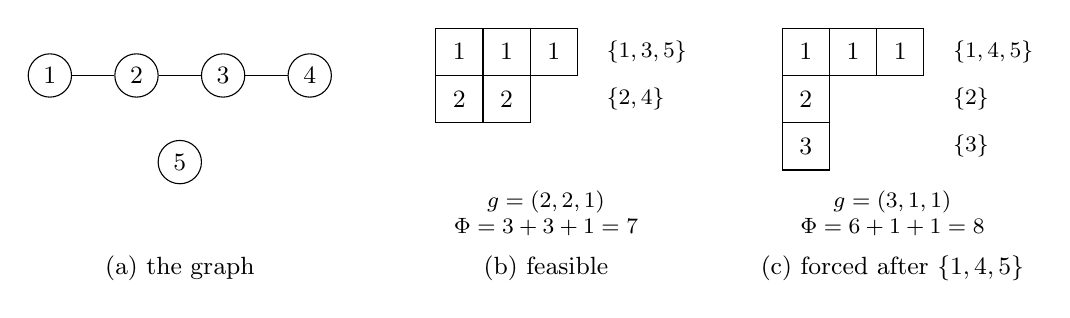
\begin{tikzpicture}[
  vtx/.style={circle,draw,inner sep=1.3pt,minimum size=5.5mm,font=\small},
  cell/.style={draw,minimum size=6mm,inner sep=0pt,font=\small}]
  % the graph
  \node[vtx] (v1) at (0,0) {1};
  \node[vtx] (v2) at (1.1,0) {2};
  \node[vtx] (v3) at (2.2,0) {3};
  \node[vtx] (v4) at (3.3,0) {4};
  \node[vtx] (v5) at (1.65,-1.1) {5};
  \draw (v1)--(v2)--(v3)--(v4);
  \node[font=\small] at (1.65,-2.45) {(a) the graph};
  % coloring (b): classes {1,3,5},{2,4}
  \begin{scope}[xshift=5.2cm,yshift=0.3cm]
    \foreach \x in {0,1,2} \node[cell] at (0.6*\x,0) {1};
    \foreach \x in {0,1} \node[cell] at (0.6*\x,-0.6) {2};
    \node[font=\footnotesize,anchor=west] at (1.75,0) {$\{1,3,5\}$};
    \node[font=\footnotesize,anchor=west] at (1.75,-0.6) {$\{2,4\}$};
    \node[font=\footnotesize,align=center] at (1.1,-2.05)
      {$g=(2,2,1)$\\ $\Phi=3+3+1=7$};
    \node[font=\small] at (1.1,-2.75) {(b) feasible};
  \end{scope}
  % coloring (c): classes {1,4,5},{2},{3}
  \begin{scope}[xshift=9.6cm,yshift=0.3cm]
    \foreach \x in {0,1,2} \node[cell] at (0.6*\x,0) {1};
    \node[cell] at (0,-0.6) {2};
    \node[cell] at (0,-1.2) {3};
    \node[font=\footnotesize,anchor=west] at (1.75,0) {$\{1,4,5\}$};
    \node[font=\footnotesize,anchor=west] at (1.75,-0.6) {$\{2\}$};
    \node[font=\footnotesize,anchor=west] at (1.75,-1.2) {$\{3\}$};
    \node[font=\footnotesize,align=center] at (1.1,-2.05)
      {$g=(3,1,1)$\\ $\Phi=6+1+1=8$};
    \node[font=\small] at (1.1,-2.75) {(c) forced after $\{1,4,5\}$};
  \end{scope}
\end{tikzpicture}
\caption{Profiles forget which vertices form the classes. For the graph (a),
each Ferrers diagram has one row per class, labelled by its color, so the
row sums give the objective class by class and the column sums are the
triangular numbers $T(g_t)$. The profile $(3,2)$ is realized with the
size-3 class $\{1,3,5\}$ (b), but not with the size-3 class $\{1,4,5\}$,
which leaves the adjacent vertices 2 and 3 as singletons (c).}
\label{fig:five-vertex}
\end{figure}

\Cref{fig:five-vertex} shows what a profile forgets. The graph has vertices
$1,\ldots,5$ and edges $12$, $23$, $34$. Its maximum stable sets are
$\{1,3,5\}$, $\{1,4,5\}$ and $\{2,4,5\}$. With the classes $\{1,3,5\}$ and
$\{2,4\}$ the profile is $\lambda=(3,2)$, with $h=(0,1,1)$, $g=(2,2,1)$ and
$\Phi(h)=T(2)+T(2)+T(1)=7$; the maximum class $\{2,4,5\}$ also admits it,
with the pair $\{1,3\}$. If the maximum class is $\{1,4,5\}$, however, the
remaining vertices $2$ and $3$ are adjacent, the profile becomes $(3,1,1)$
and the sum is $8$. A bound that records only how many classes of size three
can occur cannot tell these cases apart. A bound that conditions on the
identity of the size-three class can, and that is the device developed in
\cref{sec:conditioning}.

\subsection{Feasibility as a packing problem}

Let $\Stable_s$ be the family of stable sets of size $s$ in $G$. Singletons
impose no compatibility condition, so they can be removed from the
combinatorial core of the problem.

\begin{proposition}[Singleton completion]
\label{prop:singleton}
A nonnegative integer profile $h=(h_1,\ldots,h_\alpha)$ with
$\sum_s s\,h_s=n$ is feasible if and only if there are pairwise-disjoint stable
sets consisting of exactly $h_s$ members of $\Stable_s$ for each $s\ge2$.
The uncovered vertices then form the singleton classes, and there are exactly
$h_1$ of them.
\end{proposition}

\begin{proof}
The classes of size at least two in a coloring with profile $h$ form such a
packing. Conversely, a packing with these counts covers $\sum_{s\ge2}s\,h_s$
vertices, so by \eqref{eq:mass} it leaves $h_1$ uncovered vertices, each a
stable singleton.
\end{proof}

Feasibility of $h$ is thus the typed set-packing system
\[
  \sum_{Q\in\Stable_s}x_Q=h_s\quad(s=2,\ldots,\alpha),\qquad
  \sum_{Q\ni v}x_Q\le1\quad(v\in V),\qquad
  x_Q\in\{0,1\}.
\]
Relaxing an equality to an upper bound enlarges the set of packings, so an
upper bound on packings proved under the relaxed counts remains valid; we use
this repeatedly.

\subsection{The stable-set master}
\label{sec:master}

Let $\Stable$ be the family of all nonempty stable sets of $G$. The integer
master has a binary variable $x_S$ for each $S\in\Stable$ and the exact-cover
constraints
\begin{equation}
  \sum_{S\ni v}x_S=1\qquad(v\in V).
  \label{eq:master-cover}
\end{equation}
For each threshold $t$ put $q_t=\sum_{S:\,|S|\ge t}x_S$. An integral solution
is a partition of $V$ into stable classes, $q_t=g_t$ counts its classes of
size at least $t$, and by \cref{prop:ferrers} its cost after canonical
relabeling is $\sum_tT(q_t)$. Conversely, every proper coloring gives an
integral solution. The integer master is therefore equivalent to MSCP.

To obtain a linear model, put $N_t=\lfloor n/t\rfloor$ and introduce unit
cells $0\le u_{t,j}\le1$ for $1\le j\le N_t$:
\begin{equation}
  \sum_{j=1}^{N_t}u_{t,j}=q_t\quad(1\le t\le\alpha),\qquad
  \text{minimize}\ \sum_{t=1}^{\alpha}\sum_{j=1}^{N_t}j\,u_{t,j}.
  \label{eq:unit-cell-master}
\end{equation}
For integral $q_t$ the cheapest $q_t$ cells are filled and the row costs
exactly $T(q_t)$. For fractional $q_t\in[0,N_t]$ it costs
$T(\lfloor q_t\rfloor)+(\lfloor q_t\rfloor+1)(q_t-\lfloor q_t\rfloor)$, the
piecewise-linear interpolation of $T$ rather than $q_t(q_t+1)/2$. Relaxing
$x_S$ to $0\le x_S\le1$ gives the \emph{master relaxation}, in which the
coordinates $q_t$ may be fractional; its value, rounded up, is a lower bound
on $\Sigma(G)$.

This is a stable-set formulation in the tradition of Mehrotra and
Trick~\cite{mehrotra1996}. Delle Donne et al.~\cite{delledonne2021} give each
pair of a stable set and a color its own variable; here the colors are
aggregated into Ferrers thresholds and the triangular cost is linearized by
unit cells. Two facts are used throughout. A rational dual solution that is
feasible for every column certifies a lower bound on the relaxation by weak
duality, and a rational primal solution of the same value certifies the
optimum. A floating-point objective or a solver's status carries neither
implication.

For \DSJCThousand{} and \CTwoThousand{} we bound or compute the optimum of
this relaxation directly (\cref{sec:larger}); for \DSJCFiveHundred{} we show
that its conditioned form cannot exclude the lowest remaining cases
(\cref{sec:dsjc500-limits}). The conditional arguments of
\cref{sec:conditioning,sec:dsjc250,sec:dsjc500} bound integer packings
directly.

\section{Conditioning on the largest classes}
\label{sec:conditioning}

Throughout, $B$ is one less than the value of a known coloring. To prove that
the coloring is optimal, or to bound how far it is from optimal, we exclude
colorings of value at most $B$. Profiles of value exactly $B$ must still be
excluded, so a bound removes a profile only when it is strictly greater than
$B$. Choosing $B$ from a known coloring assumes nothing about optimality.

\subsection{Top packings, cells and envelopes}
\label{sec:envelope-defs}

\begin{definition}
\label{def:envelope}
A \emph{top packing} is a family $F$ of pairwise-disjoint stable sets of size
$\alpha$. A coloring \emph{has top packing $F$} if its classes of size
$\alpha$ are exactly the members of $F$. Every coloring has exactly one top
packing, which may be empty; other stable $\alpha$-sets may exist in
$G-\bigcup F$, but in a coloring with top packing $F$ none of them is a color
class. A \emph{cell} is a pair $(F,h)$ of a top packing and a profile with
$h_\alpha=|F|$.

Fix a top packing $F$ and a set $E\subseteq\{2,\ldots,\alpha-1\}$ of
\emph{eligible sizes}. The \emph{complete residual universe} is
\[
  \Res_F(E)=\Bigl\{Q\subseteq V\setminus\textstyle\bigcup F:\
  Q\text{ is stable and }|Q|\in E\Bigr\},
\]
and a \emph{residual packing} is a pairwise-disjoint subfamily
$\mathcal A\subseteq\Res_F(E)$, with $n_s(\mathcal A)$ members of size $s$.
Given prescribed numbers of residual classes of each size above $s$, the
\emph{conditional envelope} at size $s$ is the largest number of $s$-sets in a
residual packing with those numbers.
\end{definition}

A cell whose profile asks for more $s$-classes than the envelope allows is
infeasible. The next proposition states the form in which we use this. It
allows several sizes to be scored at once, which is how envelopes given
counts at larger sizes are certified (\cref{sec:lexicographic}).

\begin{proposition}[Conditional exclusion]
\label{prop:conditional-exclusion}
Let $F$ be a top packing, $E$ a set of eligible sizes with scores $a_s>0$,
$c_s$ caps on some of the sizes in $E$, and $\tau$ an integer. Suppose every
residual packing $\mathcal A\subseteq\Res_F(E)$ with $n_s(\mathcal A)\le c_s$
for each capped size satisfies $\sum_{Q\in\mathcal A}a_{|Q|}<\tau$. Then no
coloring with top packing $F$ has residual class counts $n_s$ $(s\in E)$ with
$n_s\le c_s$ for each capped size and $\sum_{s\in E}a_sn_s\ge\tau$.
\end{proposition}

\begin{proof}
The classes of such a coloring whose sizes lie in $E$ are stable, pairwise
disjoint and disjoint from $\bigcup F$, so they lie in $\Res_F(E)$ and form a
residual packing that respects the caps and scores at least $\tau$, a
contradiction. Classes of other sizes are simply ignored, which can only
enlarge the family of packings considered.
\end{proof}

The hypothesis that $\Res_F(E)$ contains \emph{every} eligible stable set is
essential: a coloring could otherwise use a class that the model omits. This
is why every residual universe in this paper is regenerated from the graph
rather than supplied as a list.

\subsection{Dual certificates}
\label{sec:dual-certificates}

Packing bounds are certified by the following form of weak duality, written
with integer data so that it can be checked without rounding.

\begin{lemma}[Scaled dual bound]
\label{lem:scaled-dual}
Let $\mathcal Q$ be a family of stable sets with scores $a_s>0$ for the sizes
that occur in it. For each size $s$ let the number $n_s(\mathcal A)$ of
members of size $s$ in a subfamily $\mathcal A$ be either unrestricted,
bounded ($n_s\le c_s$) or fixed ($n_s=c_s$). Let $D$ be a positive integer,
$y_v\ge0$ integer vertex weights, and $\mu_s$ integers with $\mu_s=0$ for
unrestricted sizes, $\mu_s\ge0$ for bounded sizes and $\mu_s$ of either sign
for fixed sizes. If
\begin{equation}
\label{eq:dual-cover}
  \sum_{v\in Q}y_v+\mu_{|Q|}\ \ge\ D\,a_{|Q|}\qquad(Q\in\mathcal Q),
\end{equation}
then every pairwise-disjoint subfamily $\mathcal A\subseteq\mathcal Q$ that
meets the count conditions satisfies
\begin{equation}
\label{eq:dual-bound}
  D\sum_{Q\in\mathcal A}a_{|Q|}\ \le\ \sum_{v}y_v+\sum_s\mu_sc_s.
\end{equation}
\end{lemma}

\begin{proof}
Sum \eqref{eq:dual-cover} over $\mathcal A$. By disjointness each
nonnegative weight $y_v$ is counted at most once. The multiplier terms sum to
$\sum_s\mu_sn_s(\mathcal A)$; on fixed sizes this equals $\mu_sc_s$, on
bounded sizes it is at most $\mu_sc_s$ because $\mu_s\ge0$, and on
unrestricted sizes it vanishes.
\end{proof}

The scores and count bounds used here are integers. Thus
\eqref{eq:dual-cover} is checked set by set and \eqref{eq:dual-bound} is
evaluated exactly; any floor is taken only after
the scaled inequality has been established. With unit scores on the sizes at
least $t$, the left side of \eqref{eq:dual-bound} is $D$ times the number of
classes of size at least $t$. For example, the global 4-set certificate for
\DSJCTwoFifty{} (S1 in \cref{app:dsjc250-data}) has $D=26$ and
$\sum_vy_v=1039$ and no count multipliers. It is checked against all 205
stable 4-sets and all three stable 5-sets of the graph, and it gives
$26g_4\le1039$, hence $g_4\le\lfloor1039/26\rfloor=39$.

This is the same principle as the safe column generation of Held, Cook and
Sewell~\cite{held2012}, who scale a floating-point dual solution to integers
and certify the scaled solution by an exact computation. In our setting the
certification is a direct check against every column of an enumerated family.

When some columns have already been selected, the lemma gives a test for
closing a case.

\begin{corollary}[Leaf test]
\label{cor:leaf}
Suppose columns of total score $p$ have been selected, let $\mathcal Q'$ be
the columns disjoint from them that remain available, and let $c'_s$ be the
remaining caps. If a certificate for $\mathcal Q'$ and $c'$ as in
\cref{lem:scaled-dual}, with $\mu_s\ge0$ for capped and $\mu_s=0$ for
uncapped sizes, satisfies
\begin{equation}
\label{eq:strict-leaf}
  Dp+\sum_vy_v+\sum_sc'_s\mu_s<D\tau,
\end{equation}
then no packing that extends the selection reaches score $\tau$.
\end{corollary}

The strict inequality \eqref{eq:strict-leaf} is checked as written, without
division or rounding. A single certificate is the special case with nothing
selected and $p=0$.

\subsection{Lexicographic scores}
\label{sec:lexicographic}

An envelope asks for the largest number of $s$-sets given the counts at
larger sizes. We certify it with one score that ranks larger sizes first. Let
$\rho=|V|+1$. Every residual count is at most $|V|<\rho$, and
$\rho^2>|V|\rho+|V|$, so one unit in a higher coordinate outweighs any
variation in the lower ones. Hence
\[
  Z_3=\rho\,n_4+n_3\qquad\text{and}\qquad Z_2=\rho^2n_4+\rho\,n_3+n_2
\]
order packings lexicographically by $(n_4,n_3)$ and by $(n_4,n_3,n_2)$,
exactly and without tolerances. For example, if every packing with
$n_4\le37$ has $Z_3<37\rho+30$, then a packing with $37$ residual 4-sets has
at most $29$ residual 3-sets. We use $\rho=251$ for \DSJCTwoFifty{} and
$\rho=501$ for \DSJCFiveHundred{}.

\subsection{Branch trees}
\label{sec:trees}

When one certificate is not strong enough, we branch. A node records the
columns selected so far, their score $p$, the active columns (those disjoint
from the selection and not excluded) and the remaining caps. An internal node
branches on an active column $Q$. Its zero child excludes $Q$; its one child
selects $Q$, adds its score, decrements the remaining quota of $|Q|$ when that
size is capped, and removes every active column that meets $Q$, which is valid
because the other members of a packing
containing $Q$ are disjoint from it. A tree is \emph{admissible} for a target
$\tau$ if its root holds the complete residual universe with the model's
caps and $p=0$, every internal node branches on an active column and has both
children, every node has valid nonnegative remaining quotas, and every leaf
passes the test of \cref{cor:leaf}.

\begin{proposition}[Soundness of trees]
\label{prop:tree-soundness}
If a tree is admissible for the target $\tau$, then no residual packing of
its model reaches score $\tau$.
\end{proposition}

\begin{proof}
Every packing represented at an internal node either omits the branching
column, and is represented at the zero child, or contains it, and is
represented at the one child after the conflicting columns are removed. Each
leaf excludes all packings it represents, so by induction from the leaves the
root excludes every packing of the model.
\end{proof}

The six \DSJCTwoFifty{} trees have at most $1{,}661$ nodes
(\cref{tab:tree-stats}). General certificate formats for integer programming
represent the same kind of case analysis differently. VIPR~\cite{cheung2017}
flattens a branch-and-bound tree into a sequence of derived inequalities,
introducing each branching disjunction as a pair of assumptions and
discharging them by `unsplitting'; Larrosa et al.~\cite{larrosa2011} separate
branch-and-bound search from its verification through checkable reasons for
each bound closure. Our trees need a single inference at the leaves, the
bound of \cref{lem:scaled-dual}, because each leaf is closed by a packing
dual checked against an explicit column family.

\section{The chromatic sum of \DSJCTwoFifty{}}
\label{sec:dsjc250}

This section proves $\Sigma(\DSJCTwoFifty)=8{,}277$. The argument has the
shape shown in \cref{fig:dsjc250-tree}. An improving coloring has at most two
5-classes, because at most two maximum stable sets are disjoint. Profile
arithmetic and bounds on the 4-set layer, some of them conditioned on the
choice of 5-class, leave 16 candidate profiles, seven with one 5-class and
nine with two. For each possible choice
of 5-classes we then bound how many 4-sets, and then 3-sets and 2-sets, fit
into the remaining vertices, and every candidate asks for more than its
choice allows.

\begin{figure}[tbp]
\centering
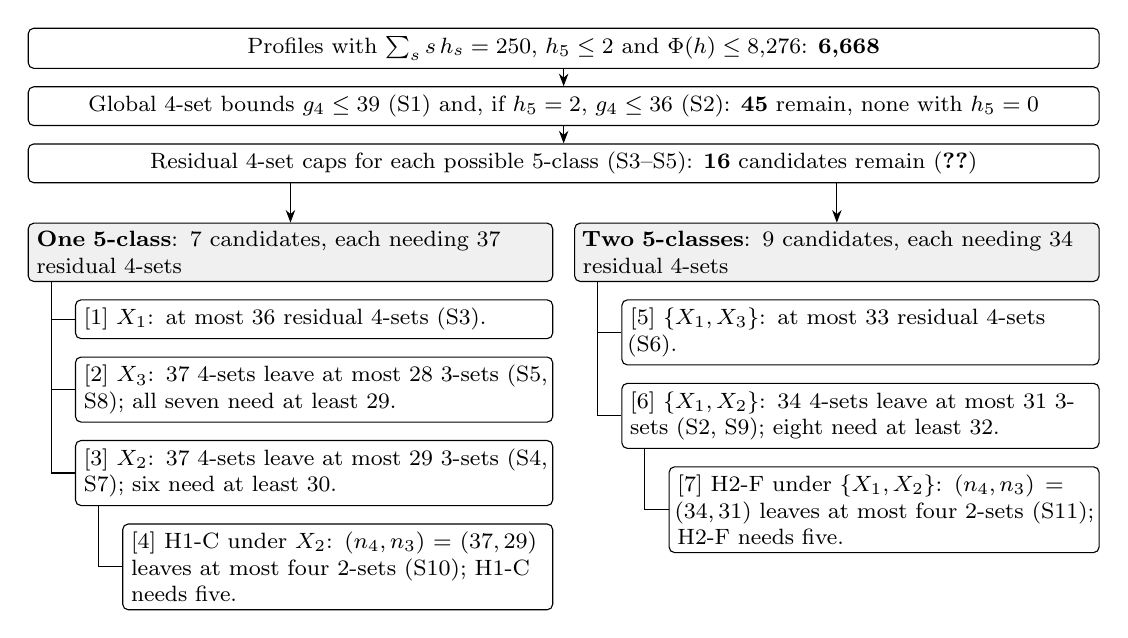
\begin{tikzpicture}[
  box/.style={draw,rounded corners=2pt,font=\footnotesize,inner sep=3pt},
  wide/.style={box,minimum width=13.6cm,align=center},
  head/.style={box,text width=6.45cm,align=left,fill=black!6},
  leaf/.style={box,text width=5.85cm,align=left},
  leafii/.style={box,text width=5.25cm,align=left},
  node distance=2.2mm and 0mm]
  \node[wide] (a) {Profiles with $\sum_s s\,h_s=250$, $h_5\le2$ and
    $\Phi(h)\le8{,}276$: \textbf{6,668}};
  \node[wide,below=of a] (b) {Global 4-set bounds $g_4\le39$ (S1) and, if
    $h_5=2$, $g_4\le36$ (S2): \textbf{45} remain, none with $h_5=0$};
  \node[wide,below=of b] (c) {Residual 4-set caps for each possible 5-class
    (S3--S5): \textbf{16} candidates remain (\cref{tab:frontier-full})};
  \node[head,below=5mm of c.south west,anchor=north west] (L)
    {\textbf{One 5-class}: 7 candidates, each needing 37 residual 4-sets};
  \node[head,below=5mm of c.south east,anchor=north east] (R)
    {\textbf{Two 5-classes}: 9 candidates, each needing 34 residual 4-sets};
  \node[leaf,below=of L.south east,anchor=north east] (l1)
    {[1] $X_1$: at most 36 residual 4-sets (S3).};
  \node[leaf,below=of l1] (l2)
    {[2] $X_3$: 37 4-sets leave at most 28 3-sets (S5, S8); all seven need
    at least 29.};
  \node[leaf,below=of l2] (l3)
    {[3] $X_2$: 37 4-sets leave at most 29 3-sets (S4, S7); six need at
    least 30.};
  \node[leafii,below=of l3.south east,anchor=north east] (l4)
    {[4] H1-C under $X_2$: $(n_4,n_3)=(37,29)$ leaves at most four 2-sets
    (S10); H1-C needs five.};
  \node[leaf,below=of R.south east,anchor=north east] (r1)
    {[5] $\{X_1,X_3\}$: at most 33 residual 4-sets (S6).};
  \node[leaf,below=of r1] (r2)
    {[6] $\{X_1,X_2\}$: 34 4-sets leave at most 31 3-sets (S2, S9); eight
    need at least 32.};
  \node[leafii,below=of r2.south east,anchor=north east] (r3)
    {[7] H2-F under $\{X_1,X_2\}$: $(n_4,n_3)=(34,31)$ leaves at most four
    2-sets (S11); H2-F needs five.};
  \draw[-{Stealth[length=1.6mm]}] (a) -- (b);
  \draw[-{Stealth[length=1.6mm]}] (b) -- (c);
  \draw[-{Stealth[length=1.6mm]}] (c.south -| L.north) -- (L.north);
  \draw[-{Stealth[length=1.6mm]}] (c.south -| R.north) -- (R.north);
  \foreach \n in {l1,l2,l3} \draw ([xshift=3mm]L.south west) |- (\n.west);
  \draw ([xshift=3mm]l3.south west) |- (l4.west);
  \foreach \n in {r1,r2} \draw ([xshift=3mm]R.south west) |- (\n.west);
  \draw ([xshift=3mm]r2.south west) |- (r3.west);
\end{tikzpicture}
\caption{The proof that no coloring of \DSJCTwoFifty{} has sum at most
$8{,}276$. Bracketed numbers are the branches of \cref{tab:branch-obligations};
S1--S11 are the certificates of \cref{tab:certificate-obligations}. $X_1$,
$X_2$, $X_3$ are the three maximum stable sets.}
\label{fig:dsjc250-tree}
\end{figure}

\subsection{The graph, a coloring of sum 8,277, and the maximum stable sets}
\label{sec:dsjc250-graph}

\DSJCTwoFifty{} has $250$ vertices and $27{,}897$ edges. \Cref{app:witnesses}
lists a coloring with $73$ classes: every vertex receives one label, the
labels $1,\ldots,73$ are all used, and no edge joins two vertices with the
same label. Its profiles are
\begin{equation}
\label{eq:incumbent-profile}
  h=(2,4,29,37,1),\qquad g=(73,71,67,38,1),
\end{equation}
so by \cref{prop:ferrers} its sum is
\begin{equation}
\label{eq:incumbent-sum}
  \Phi(h)=T(73)+T(71)+T(67)+T(38)+T(1)=2701+2556+2278+741+1=8277.
\end{equation}
Hence $\Sigma(\DSJCTwoFifty)\le8{,}277$, and we take $B=8{,}276$.

Enumerating the stable sets in increasing vertex order gives
\[
 (|\Stable_1|,\ldots,|\Stable_6|)=(250,\ 3{,}228,\ 2{,}869,\ 205,\ 3,\ 0).
\]
There is no stable 6-set, so $\alpha=5$, and there are exactly three stable
5-sets:
\[
  X_1=\{3,69,88,154,223\},\qquad
  X_2=\{4,51,121,189,247\},\qquad
  X_3=\{67,119,166,189,247\}.
\]
$X_1$ is disjoint from $X_2$ and from $X_3$, while $X_2\cap X_3=\{189,247\}$.
The top packing of any coloring is therefore one of $\emptyset$, $\{X_1\}$,
$\{X_2\}$, $\{X_3\}$, $\{X_1,X_2\}$ and $\{X_1,X_3\}$, and at most two
5-classes can occur; two is the cap of Gondran et al.~\cite{gondran2019} for
this graph. The coloring above has the single 5-class $X_2$.

\subsection{Profiles that could improve on 8,277}
\label{sec:profile-enumeration}

By \cref{cor:ferrers-lower,prop:singleton}, a coloring of sum at most
$8{,}276$ has an exact-size profile $h=(h_1,\ldots,h_5)$ of nonnegative
integers with
\begin{equation}
\label{eq:threshold-system}
  \sum_{s=1}^5 s\,h_s=250,\qquad h_5\le2,\qquad \Phi(h)\le8{,}276.
\end{equation}
Listing the integer solutions is a finite calculation: there are $6{,}668$ of
them. \Cref{tab:profile-reduction} shows how they are distributed over $h_5$
and how the next two steps reduce them.

\begin{table}[t]
\centering
\caption{Reduction of the improving profiles of \DSJCTwoFifty{}. The last
row applies, for each possible choice of 5-classes, the residual 4-set bounds
of \cref{tab:capacities}.}
\label{tab:profile-reduction}
\begin{tabular}{@{}lrrrr@{}}
\toprule
stage & total & $h_5=0$ & $h_5=1$ & $h_5=2$\\
\midrule
profiles with $\Phi(h)\le 8{,}276$ & 6,668 & 1,741 & 2,208 & 2,719 \\
$g_4\le39$; if $h_5=2$, $g_4\le36$ (S1, S2) & 45 & 0 & 36 & 9 \\
residual 4-set caps for each top packing & 16 & 0 & 7 & 9
\tabularnewline
\bottomrule
\end{tabular}
\end{table}

\subsection{The 4-set layer}
\label{sec:fourth-layer}

Let $g_4=h_4+h_5$ be the number of classes of size at least four. The
certificate S1 described after \cref{lem:scaled-dual} gives $g_4\le39$ for
every coloring, and \cref{app:witnesses} lists $39$ pairwise-disjoint stable
4-sets, so $39$ is the exact maximum. A second certificate, S2, uses a
multiplier for the fixed count $h_5=2$; with $D=2$ and right-hand side $73$
it gives $2g_4\le73$, so $g_4\le36$ when there are two 5-classes. Both
certificates are checked against every stable 4- and 5-set, and in both the
minimum slack is zero.

These two bounds leave $45$ of the $6{,}668$ profiles. None has $h_5=0$. With
$g_5=0$ and $g_4\le39$, the cost is least when the first three Ferrers
coordinates are balanced, at $g=(71,70,70,39,0)$, where
$\Phi=8{,}306>8{,}276$; so a profile with $h_5=0$ would need $g_4\ge40$. Of
the $36$ survivors with one 5-class, $29$ have $(h_4,h_5)=(38,1)$ and hence
$g_4=39$, and seven have $(h_4,h_5)=(37,1)$ and $g_4=38$. The nine with two
5-classes all have $(h_4,h_5)=(34,2)$.

Conditioning first pays off at this layer. \Cref{tab:capacities} lists what
fits below each top packing. If $X_1$ is the only 5-class, at most $36$
disjoint 4-sets fit in the remaining vertices (S3), so $g_4\le37$. If it is
$X_2$ or $X_3$, at most $37$ fit (S4, S5), so $g_4\le38$. Without
conditioning the bound is $g_4\le39$, and it is attained. None of the $29$
profiles with $g_4=39$ is therefore realizable under any choice of 5-class,
while the seven with $g_4=38$ survive under $X_2$ or $X_3$. With the nine
two-class profiles, $7+9=16$ candidates remain; they are listed in
\cref{tab:frontier-full}. Every candidate with one 5-class needs $37$
residual 4-sets and every candidate with two needs $34$.

\begin{table}[t]
\centering
\small
\caption{Packing capacities of \DSJCTwoFifty{}. An entry $=k$ is attained
by an explicit packing; $\le k$ is an upper bound. The 3-set column assumes
the maximum number of residual 4-sets; the 2-set column assumes the 4- and
3-set counts required by H1-C (for $\{X_2\}$) and H2-F (for $\{X_1,X_2\}$).}
\label{tab:capacities}
\begin{tabular}{@{}lcccl@{}}
\toprule
case & 4-sets & 3-sets & 2-sets & certificates\\
\midrule
\multicolumn{5}{@{}l}{\emph{Global bounds on $g_4$, the number of classes of size at least four}}\\
all colorings & $g_4=39$ & & & S1; \cref{app:witnesses}\\
colorings with $h_5=2$ & $g_4\le36$ & & & S2\\
\midrule
\multicolumn{5}{@{}l}{\emph{Residual bounds for each top packing}}\\
$\{X_1\}$ & $\le36$ & & & S3\\
$\{X_2\}$ & $=37$ & $=29$ & $=4$ & S4, S7, S10\\
$\{X_3\}$ & $=37$ & $=28$ & & S5, S8\\
$\{X_1,X_2\}$ & $=34$ & $=31$ & $=4$ & S2, S9, S11\\
$\{X_1,X_3\}$ & $\le33$ & & & S6
\tabularnewline
\bottomrule
\end{tabular}
\end{table}

\subsection{The 3-set and 2-set layers}
\label{sec:envelopes}

For the survivors the next question is how many 3-sets fit once the required
4-sets are in place. Under $X_2$, take the eligible sizes $\{4,3\}$, the cap
$n_4\le37$ from S4, the score $Z_3=251n_4+n_3$ and the target
$37\cdot251+30=9{,}317$. An admissible tree, S7, shows that every packing
scores at most $9{,}316=37\cdot251+29$, and an explicit packing with $37$
4-sets and $29$ 3-sets attains this score. So with $37$ residual 4-sets at
most $29$ residual 3-sets fit, and $29$ is attained. The same construction
gives at most $28$ 3-sets under $X_3$ (S8: score at most
$9{,}315=37\cdot251+28$, attained by $(37,28)$) and at most $31$ 3-sets
beside $34$ 4-sets under $\{X_1,X_2\}$ (S9: score at most
$8{,}565=34\cdot251+31$, attained by $(34,31)$).

For the two candidates that survive this layer we go one step further, with
$Z_2=251^2n_4+251n_3+n_2$ and $251^2=63{,}001$. Under $X_2$ with $n_4\le37$
and $n_3\le29$, the tree S10 bounds $Z_2$ by $2{,}338{,}320$, one less than
the target $37\cdot63{,}001+29\cdot251+5=2{,}338{,}321$. So at most four
2-sets fit beside $37$ 4-sets and $29$ 3-sets, and the coloring of
\cref{app:witnesses} attains $(37,29,4)$. Under $\{X_1,X_2\}$ with
$n_4\le34$ and $n_3\le31$, S11 bounds $Z_2$ by $2{,}149{,}819$ against the
target $2{,}149{,}820$. So at most four 2-sets fit beside $34$ 4-sets and
$31$ 3-sets; this is attained by a coloring of sum $8{,}278$ with profile
$(3,4,31,34,2)$.

Every entry marked $=$ in \cref{tab:capacities} is attained by an explicit
packing. These are therefore the exact conditional maxima, not merely upper
bounds.

\subsection{The seven branches}
\label{sec:branches}

\Cref{tab:branch-obligations} lists the complete case analysis, and
\cref{fig:dsjc250-tree} draws it as a tree.

\paragraph{Candidates with one 5-class.} Each needs $37$ residual 4-sets.
Under $X_1$ at most $36$ fit (branch~1). Under $X_3$, $37$ 4-sets leave room
for at most $28$ 3-sets, while every candidate needs at least $29$
(branch~2). Under $X_2$, $37$ 4-sets leave room for at most $29$ 3-sets,
which rules out the six candidates that need $30$ or more (branch~3). The
last candidate is
\begin{equation}
\label{eq:H1C}
  \mathrm{H1\mbox{-}C}=(h_1,h_2,h_3,h_4,h_5)=(0,5,29,37,1),\qquad\Phi=8{,}276,
\end{equation}
which needs $X_2$ as its 5-class, $37$ 4-sets, $29$ 3-sets and five 2-sets;
at most four fit (branch~4).

\paragraph{Candidates with two 5-classes.} The top packing is
$\{X_1,X_2\}$ or $\{X_1,X_3\}$, and each candidate needs $34$ residual
4-sets. Under $\{X_1,X_3\}$ at most $33$ fit (branch~5). Under
$\{X_1,X_2\}$, $34$ 4-sets leave room for at most $31$ 3-sets, which rules
out the eight candidates that need $32$ or more (branch~6). The last
candidate is
\begin{equation}
\label{eq:H2F}
  \mathrm{H2\mbox{-}F}=(h_1,h_2,h_3,h_4,h_5)=(1,5,31,34,2),\qquad\Phi=8{,}276,
\end{equation}
which needs $34$ 4-sets, $31$ 3-sets and five 2-sets; at most four fit
(branch~7).

\begin{table}[t]
\centering
\small
\caption{The seven branches of the \DSJCTwoFifty{} proof. Each row is an
application of \cref{prop:conditional-exclusion} to the complete residual
universe of the stated top packing.}
\label{tab:branch-obligations}
\begin{tabularx}{\textwidth}{@{}cYYY@{}}
\toprule
branch & case & certified consequence & candidates closed\\
\midrule
1 & one 5-class, $X_1$ & S3: $n_4\le36$ & all seven (each needs $n_4=37$)\\
2 & one 5-class, $X_3$ & S5, S8: $n_4=37\Rightarrow n_3\le28$ & all seven (each needs $n_3\ge29$)\\
3 & one 5-class, $X_2$, $n_3\ge30$ & S4, S7: $n_4=37\Rightarrow n_3\le29$ & six\\
4 & H1-C under $X_2$ & S10: $(n_4,n_3)=(37,29)\Rightarrow n_2\le4$ & H1-C, which needs $n_2=5$\\
5 & two 5-classes, $\{X_1,X_3\}$ & S6: $n_4\le33$ & all nine (each needs $n_4=34$)\\
6 & two 5-classes, $\{X_1,X_2\}$, $n_3\ge32$ & S2, S9: $n_4=34\Rightarrow n_3\le31$ & eight\\
7 & H2-F under $\{X_1,X_2\}$ & S11: $(n_4,n_3)=(34,31)\Rightarrow n_2\le4$ & H2-F, which needs $n_2=5$
\tabularnewline
\bottomrule
\end{tabularx}
\end{table}

The last two branches have a transparent reading. Under H1-C the 5-class,
the $37$ 4-sets and the $29$ 3-sets cover $5+148+87=240$ vertices, and the
profile needs the remaining ten to split into five stable pairs, that is, a
perfect matching in the complement of the graph they induce. Under H2-F the
top classes, $34$ 4-sets and $31$ 3-sets cover $10+136+93=239$ vertices,
and the remaining eleven would need to form five stable pairs and a
singleton. S10 and S11 certify, by dual bounds over the whole residual
packing, that at most four pairs are available.

\begin{theorem}
\label{thm:lower}
No proper coloring of \DSJCTwoFifty{} has sum at most $8{,}276$.
\end{theorem}

\begin{proof}
By \cref{cor:ferrers-lower,prop:singleton} and the census of
\cref{sec:dsjc250-graph}, such a coloring has one of the $6{,}668$ profiles of
\cref{sec:profile-enumeration}. The certificates S1--S5, applied to every
possible top packing, reduce these to the $16$ candidates of
\cref{tab:frontier-full}, and the seven branches of
\cref{tab:branch-obligations} exclude all of them.
\end{proof}

\begin{proof}[Proof of \cref{thm:main-intro}(i)]
The coloring \eqref{eq:incumbent-sum} gives $\Sigma(\DSJCTwoFifty)\le8{,}277$,
and \cref{thm:lower} gives $\Sigma(\DSJCTwoFifty)\ge8{,}277$.
\end{proof}

\subsection{A direct solve of the master}
\label{sec:dsjc250-direct}

For this graph the integer master of \cref{sec:master} is small. It has
$255$ equations and $7{,}125$ variables: $6{,}555$ binary set variables, one
for each nonempty stable set, and $570$ continuous unit-cell variables. Two archived one-thread
runs of HiGHS~1.11.0 each reported objective and bound $8{,}277$ with zero
displayed gap, after $1{,}601$ branch-and-bound nodes and $278{,}786$ LP
iterations. Both returned the same $73$-class coloring, which we checked
independently to have profile $(2,4,29,37,1)$ and sum $8{,}277$. The model's
column universe and coefficients were also checked independently.

The runs agree with \cref{thm:lower} but do not prove it: the solver works in
floating point, and the archive holds no independently replayable record of
its lower bound. The argument of this section supplies such a proof, and one
whose structure a reader can follow. Eleven certificates in seven branches
show that under every choice of 5-classes the remaining vertices lack room
for the 4-, 3- or 2-sets an improving profile needs. The archived runs are
described further in \cref{app:highs}.

\section{\DSJCFiveHundred{}: how far conditioning goes}
\label{sec:dsjc500}

For \DSJCFiveHundred{} the same approach proves the lower bound $29{,}791$
but leaves an interval. The three cases at its lower end show where
reasoning about the conditioned relaxation stops.

\subsection{The graph, a coloring and the top packings}

The census of \DSJCFiveHundred{} is in \cref{tab:dsjc500-instance}. Its
DIMACS file declares $224{,}874$ edges and lists $112{,}437$ distinct
undirected edges, a documented doubled-header convention
(\cref{app:files}). There are $23$ stable 5-sets and no stable 6-set, so
$\alpha=5$. At most $15$ of the 5-sets are pairwise disjoint, and exactly
eight families of $15$ disjoint 5-sets exist; we number them P1--P8 in the
deterministic order used by the checking programs.

\begin{table}[t]
\centering
\caption{Stable sets, top packings and the coloring of sum $29{,}848$ for
\DSJCFiveHundred{}.}
\label{tab:dsjc500-instance}
\begin{tabular}{@{}lr@{}}
\toprule
quantity & value\\
\midrule
vertices & 500 \\
distinct undirected edges & 112,437 \\
$(|\Stable_1|,\ldots,|\Stable_6|)$ & $(500,12{,}313,19{,}901,2{,}428,23,0)$ \\
independence number & 5 \\
maximum number of disjoint stable $5$-sets & 15 \\
number of maximum $5$-set packings & 8 \\
profile $(h_1,\ldots,h_5)$ of the coloring & $(3,4,10,96,15)$ \\
classes / sum of the coloring & $128\;/\;29{,}848$
\tabularnewline
\bottomrule
\end{tabular}
\end{table}

A coloring with $128$ classes has profile $(3,4,10,96,15)$ and sum
$29{,}848$; every vertex occurs once, each class is stable, and the labels are
already in nonincreasing order of class size. Its fifteen 5-classes form P5.
Every coloring of smaller sum must also have fifteen 5-classes. If
$g_5=h_5\le14$, the cost is least when the first four Ferrers coordinates are
balanced, and while $g_5\le14$ moving a unit from one of them (each at least
$121$) to $g_5$ lowers the cost. The minimum is therefore at
$g=(122,122,121,121,14)$, where
\[
  2T(122)+2T(121)+T(14)=29{,}873>29{,}847.
\]
So the top packing of an improving coloring is one of P1--P8. Each covers
$75$ vertices and leaves $425$ for classes of size at most four. Here a cell
is a pair of one of these packings and a profile; the same profile under two
packings gives two cells.

\subsection{Excluding cells}
\label{sec:dsjc500-exclusions}

Set $B=29{,}847$. Graph-free enumeration gives $230$ profiles with
$\Phi(h)\le B$, all with $h_5=15$. Residual 4-set certificates give
$h_4\le101$ under each of the eight packings, which leaves $160$ profiles per
packing, $1{,}280$ cells in all. Farkas certificates exclude the profile
$(0,0,7,101,15)$ under each of the eight packings and three further cells,
leaving $1{,}269$. Two further 4-set trees sharpen the bound to $h_4\le100$
under P2 and P4, removing $74$ cells.

Seventeen conditional trees then exclude $30$ more cells, each through an
explicit implication from a cell to a model of
\cref{prop:conditional-exclusion}. The implication checks the top packing,
the complete residual universe, the caps and the score that the cell
requires. For example, under the caps $h_4\le101$ and $h_3\le6$, a profile
with $(h_4,h_3)=(101,6)$ has score $501h_4+h_3=50{,}607$, and a tree showing
that every compatible residual packing scores less excludes it. Other trees
also carry the simultaneous demand for pairs where it is needed.
\Cref{tab:dsjc500-reduction} summarizes the reduction; $1{,}165$ cells remain.
(A one-way splitting organization of these cells, which no exclusion uses, is
described in \cref{app:splitting}.)

\begin{table}[t]
\centering
\caption{Exclusion of cells for \DSJCFiveHundred{}.}
\label{tab:dsjc500-reduction}
\begin{tabular}{@{}lrr@{}}
\toprule
stage & removed & remaining\\
\midrule
graph-free profiles with $\Phi(h)\le29{,}847$, all with $h_5=15$ & -- & 230 profiles \\
residual bound $h_4\le101$ under each of P1--P8 & -- & $8\times160=1{,}280$ cells \\
Farkas certificates & 11 & 1,269 \\
$h_4\le100$ under P2 and P4 (two trees) & 74 & 1,195 \\
conditional trees (17 trees) & 30 & 1,165
\tabularnewline
\bottomrule
\end{tabular}
\end{table}

\subsection{The lower bound}

Every cell of value at most $29{,}790$ is excluded, and exactly three cells
remain at $29{,}791$ (\cref{tab:dsjc500-endpoints}). Profile arithmetic alone
does not give this value: the graph-free profiles with $\Phi(h)\le B$ take
every value from $29{,}766$ to $29{,}847$. Those of value $29{,}789$ and
$29{,}790$ all have $h_4\ge102$ and are removed by the residual bound
$h_4\le101$, and among the profiles with $h_4\le101$ no value lies strictly
between $29{,}788$ and $29{,}791$.

\begin{table}[t]
\centering
\caption{The three remaining \DSJCFiveHundred{} cells of value $29{,}791$.}
\label{tab:dsjc500-endpoints}
\begin{tabular}{@{}ccr@{}}
\toprule
top packing & $(h_1,h_2,h_3,h_4,h_5)$ & $\Phi(h)$\\
\midrule
P5 & $(1,4,4,101,15)$ & 29,791 \\
P5 & $(4,1,5,101,15)$ & 29,791 \\
P7 & $(4,1,5,101,15)$ & 29,791
\tabularnewline
\bottomrule
\end{tabular}
\end{table}

\begin{theorem}
\label{thm:dsjc500-interval}
$29{,}791\le\Sigma(\DSJCFiveHundred)\le29{,}848$.
\end{theorem}

\begin{proof}
The coloring above gives the upper bound. A coloring of smaller sum has one
of P1--P8 as its top packing and one of the enumerated profiles, and the
certificates of \cref{sec:dsjc500-exclusions} exclude every such cell of
value at most $29{,}790$.
\end{proof}

This proves \cref{thm:main-intro}(ii). Of the $1{,}165$ remaining cells,
three have value $29{,}791$ and $1{,}162$ have values from $29{,}792$ to
$29{,}847$. Excluding the three lowest would raise the lower bound to
$29{,}792$. The census decides neither whether $29{,}791$ is attained nor
whether the coloring of sum $29{,}848$ is optimal. \Cref{app:neighbourhood}
records a separate certificate about that coloring: every improving coloring
must change at least one of its 5- or 4-classes.

\subsection{Why the three lowest cells resist}
\label{sec:dsjc500-limits}

The three endpoint cells need joint residual packings. Under P5 or P7,
$101$ residual 4-sets must coexist with four 3-sets and four 2-sets, or with
five 3-sets and one 2-set. The difficulty lies in the identities and
compatibility of several layers at once, not in the number of 4-sets alone.

A continuous model shows that no argument valid for the conditioned
relaxation can exclude these cells. Fix the top packing $P$ of a cell, let
$R=V\setminus\bigcup_{S\in P}S$, and let $\Stable_s(R)$ be the family of
stable $s$-sets of $G[R]$. For the cell's counts $(h_2,h_3,h_4)$ consider
\begin{equation}
\begin{aligned}
 x_S&\ge0 &&\bigl(S\in\Stable_2(R)\cup\Stable_3(R)\cup\Stable_4(R)\bigr),\\
 \sum_{S\ni v}x_S&\le1 &&(v\in R),\\
 \sum_{S\in\Stable_s(R)}x_S&=h_s &&(s=2,3,4).
\end{aligned}
\label{eq:dsjc500-continuous-profile}
\end{equation}
Given a solution, give each residual vertex the singleton weight
$1-\sum_{S\ni v}x_S$. These weights are nonnegative and sum to
$425-2h_2-3h_3-4h_4=h_1$, so together with the top packing they satisfy the
covering equations of the master relaxation conditioned on $P$. The class
totals are integral even though the column weights need not be, so the
Ferrers coordinates are those of the cell and the unit-cell objective is
exactly $\Phi(h)=29{,}791$.

Explicit rational solutions of \eqref{eq:dsjc500-continuous-profile} exist
for P5 with $(h_2,h_3,h_4)=(4,4,101)$, and for P5 and for P7 with
$(h_2,h_3,h_4)=(1,5,101)$. Their checks reconstruct the graph and the
packings, verify that every column in the support is a stable residual set,
and recompute the vertex loads, the class totals and the singleton deficits
exactly (\cref{app:replay}). Hence no inequality valid for this continuous
model excludes the three cells. Excluding them requires information of
another kind, such as integrality of the residual packing, a disjunction or
branching, or a valid inequality for the integer hull. The rational points
establish continuous feasibility only; they are not colorings, and they do
not rule out stronger relaxations.

\section{The master relaxation: \DSJCThousand{} and \CTwoThousand{}}
\label{sec:larger}

For the two larger graphs $\alpha=6$, and we use the master relaxation
of \cref{sec:master} rather than integer packings. \DSJCThousand{} has only
three stable 6-sets, so conditioning on them gives an eight-way case split
with one relaxation for each case. For \CTwoThousand{} the cap on the number
of 6-classes already gives a bound that the unconditioned relaxation attains.

\subsection{\DSJCThousand{}}
\label{sec:dsjc1000}

\DSJCThousand{} has $1{,}000$ vertices and $449{,}449$ edges. Complete
enumeration gives
\[
 (|\Stable_1|,\ldots,|\Stable_6|)=(1{,}000,\ 50{,}051,\ 167{,}104,\ 41{,}659,\ 869,\ 3)
\]
and no stable 7-set, so $\alpha=6$ and there are $260{,}686$ nonempty stable
sets. The three stable 6-sets are
\begin{align*}
 A_1&=\{52,54,175,319,501,704\},\\
 A_2&=\{76,145,184,672,793,805\},\\
 A_3&=\{129,150,181,321,456,762\},
\end{align*}
and they are pairwise disjoint, so the 6-classes of any coloring form one of
their eight subsets. Unlike the top packings of \DSJCFiveHundred{}, where the
number of 5-classes was forced to its maximum, these cases include every
number of 6-classes from zero to three.

\paragraph{The unconditioned relaxation.} A rational dual solution of the
master relaxation, checked against all $260{,}686$ columns, has value
\[
 L_{\mathrm{master}}=\frac{102308106541886}{10^9}=102{,}308.106541886,
\]
so $\Sigma(\DSJCThousand)\ge102{,}309$. This dual is feasible but not
optimal: every column inequality holds with slack at least $|S|\cdot10^{-9}$,
so raising every vertex weight by $10^{-9}$ preserves feasibility and
increases the value by $10^{-6}$. We have not computed the optimum of the
relaxation.

\paragraph{The eight conditioned relaxations.} For a mask
$b=(b_1,b_2,b_3)\in\{0,1\}^3$, select $A_i$ exactly when $b_i=1$, let
$k=b_1+b_2+b_3$, and put
\[
 R_b=V\setminus\bigcup_{i:\,b_i=1}A_i,\qquad
 \Stable_b=\{S\subseteq R_b:\ S\text{ stable},\ 1\le|S|\le5\}.
\]
An unselected $A_i$ is excluded as a whole class, but its smaller stable
subsets remain eligible, so $\Stable_b$ is the complete residual universe for
this choice of 6-classes. The leftmost bit refers to $A_1$; for example, mask
$101$ selects $A_1$ and $A_3$ and excludes $A_2$ as a class. With
$N_t=\lfloor|R_b|/t\rfloor$, the conditioned relaxation is
\begin{equation}
\begin{aligned}
 \text{minimize}\quad &6T(k)+\sum_{t=1}^{5}\sum_{j=1}^{N_t}(k+j)\,u_{t,j}\\
 \text{subject to}\quad
 &\sum_{S\in\Stable_b:\,v\in S}x_S=1 &&(v\in R_b),\\
 &r_t=\sum_{S\in\Stable_b:\,|S|\ge t}x_S=\sum_{j=1}^{N_t}u_{t,j} &&(1\le t\le5),\\
 &x_S\ge0,\qquad 0\le u_{t,j}\le1.
\end{aligned}
\label{eq:dsjc1000-conditional-master}
\end{equation}
For an integral cover, $r_t$ counts the residual classes of size at least
$t$, the full Ferrers coordinates are $q_t=k+r_t$ for $t\le5$ and $q_6=k$,
and the minimized objective over the unit cells is
\[
 6T(k)+\sum_{t=1}^{5}\bigl(kr_t+T(r_t)\bigr)=\sum_{t=1}^{6}T(q_t).
\]
The shift by $k$ accounts for the labels already taken by the $k$ selected
6-classes. For fractional $x$ the coordinates $r_t$ need not be integers,
and the model keeps the piecewise-linear unit-cell cost rather than
substituting $T(r_t)$.

Scenario $111$ receives one additional inequality. Its $982$ residual
vertices contain exactly $750$ stable 5-sets, and nonnegative rational
weights $w_v$ satisfy
\[
 \sum_{v\in S}w_v\ge1\quad(S\in\Stable_{111},\ |S|=5),
 \qquad
 \sum_{v\in R_{111}}w_v=\frac{134549891193}{10^9}<135.
\]
Summing over a disjoint family of these 5-sets shows that its integer
cardinality is strictly below $135$, hence at most $134$. Every integral
coloring in scenario $111$ therefore has at most $134$ residual 5-classes.
Thus $r_5\le134$ is an integer-valid strengthening imposed on
\eqref{eq:dsjc1000-conditional-master} for $b=111$ only. For a fractional
packing the weight vector alone gives only $r_5\le134.549891193$. The cap
concerns residual
classes; the corresponding full coordinate is $q_5=3+r_5$. Both the strict
threshold $135$ and the residual universe after all three selections are
essential to the inference.

\paragraph{Dual certificates.} Each scenario is certified by rational vertex
prices $\pi_v$ $(v\in R_b)$, slopes $\beta_t$ and a multiplier $\delta\ge0$
for the cap, with $\delta=0$ except in scenario $111$, satisfying
\begin{equation}
 \sum_{v\in S}\pi_v\le\sum_{t=1}^{|S|}\beta_t+\delta\,\mathbf 1_{\{|S|=5\}}
 \qquad(S\in\Stable_b).
\label{eq:dsjc1000-conditional-dual}
\end{equation}
Put $\Gamma_k(\beta)=\sum_{j\ge1}\max\{0,\beta-(k+j)\}$, a finite sum. The
certificates have $\beta_t\le k+N_t+1$, so the positive terms have $j\le N_t$.
Each unit cell satisfies $(k+j)u\ge\beta u-\max\{0,\beta-(k+j)\}$ for
$0\le u\le1$, so the objective of \eqref{eq:dsjc1000-conditional-master} is
at least $6T(k)+\sum_t\beta_tr_t-\sum_t\Gamma_k(\beta_t)$. By
\eqref{eq:dsjc1000-conditional-dual} and the exact cover,
$\sum_t\beta_tr_t=\sum_Sx_S\sum_{t\le|S|}\beta_t\ge\sum_v\pi_v-\delta r_5$,
and $r_5\le134$ in scenario $111$. Hence
\begin{equation}
 L_b=6T(k)+\sum_{v\in R_b}\pi_v-\sum_{t=1}^{5}\Gamma_k(\beta_t)-134\,\delta
 \label{eq:dsjc1000-scenario-bound}
\end{equation}
is a lower bound for scenario $b$, the last term being present only for
$b=111$. The certificates use the denominator $10^9$ throughout; their
inequalities are checked over all eligible residual columns and their values
are recomputed in integer arithmetic.

\begin{table}[t]
\centering
\caption{The eight cases for \DSJCThousand{}. In each, the listed 6-sets are
selected and the others among $A_1,A_2,A_3$ are excluded as classes. Every
decimal is an exact rational with denominator $10^9$; only mask $111$ uses the
cap $r_5\le134$.}
\label{tab:dsjc1000-scenarios}
\begin{tabular}{@{}clrr@{}}
\toprule
mask & selected 6-sets & $L_b$ & $\lceil L_b\rceil$\\
\midrule
$000$ & none              & $102{,}633.344579608$ & $102{,}634$\\
$001$ & $A_3$             & $102{,}513.319748705$ & $102{,}514$\\
$010$ & $A_2$             & $102{,}557.583397861$ & $102{,}558$\\
$011$ & $A_2,A_3$         & $102{,}432.711355035$ & $102{,}433$\\
$100$ & $A_1$             & $102{,}503.510602511$ & $102{,}504$\\
$101$ & $A_1,A_3$         & $102{,}395.380611244$ & $102{,}396$\\
$110$ & $A_1,A_2$         & $102{,}443.215571129$ & $102{,}444$\\
$111$ & $A_1,A_2,A_3$     & $102{,}343.581115274$ & $102{,}344$\\
\bottomrule
\end{tabular}
\end{table}

Every coloring belongs to one row of \cref{tab:dsjc1000-scenarios}, so
\[
 \Sigma(\DSJCThousand)\ge
 \left\lceil\min_{b\in\{0,1\}^3}L_b\right\rceil
 =\left\lceil\frac{102343581115274}{10^9}\right\rceil
 =102{,}344.
\]
Conditioning adds $35$ to the bound $102{,}309$ from the unconditioned dual.
Because that dual is not optimal, the $35$ measures the gain over this dual,
not over the optimum of the unconditioned relaxation.

A coloring with $225$ classes and profile
$(h_1,\ldots,h_6)=(2,4,17,74,125,3)$, checked class by class and edge by
edge, has sum $103{,}256$. Hence
\begin{equation}
 102{,}344\le\Sigma(\DSJCThousand)\le103{,}256,
 \label{eq:dsjc1000-interval}
\end{equation}
which proves \cref{thm:main-intro}(iii); the gap is $912$.

\subsection{\CTwoThousand{}}
\label{sec:c2000}

\CTwoThousand{} has $2{,}000$ vertices and $1{,}799{,}532$ distinct undirected
edges. Complete enumeration gives
\[
 (|\Stable_1|,\ldots,|\Stable_6|)
 =(2{,}000,\ 199{,}468,\ 1{,}322{,}912,\ 656{,}504,\ 26{,}224,\ 90)
\]
and no stable 7-set, so $\alpha=6$. Among the $90$ stable 6-sets the
certificate exhibits $52$ that are pairwise disjoint, and partitions all $90$
into $52$ cliques of their intersection graph. A disjoint family contains at
most one member of each clique, so the maximum is exactly $52$, and every
coloring has $h_6\le52$. (Any 52-vertex set meeting every 6-set, such as the
set $Z$ used below, yields such a partition: group the 6-sets according to a
vertex of $Z$ that they contain.)

\paragraph{The profile bound.} With $\alpha=6$ and at most $52$ classes of
size six, the profile relaxation of Gondran et
al.~\cite[Sections~2.2--2.3]{gondran2019} gives the lower bound. For fixed
$g_6=m\le52$ the first five Ferrers coordinates sum to $2000-m$, and by
convexity of $T$ their contribution is least when they differ by at most one.
Increasing $m$ towards $52$ lowers the total, since it moves a unit from a
coordinate of size at least $389$ to one of size at most $52$. The unique
minimizer is
\[
  g=(390,390,390,389,389,52),\qquad h=(0,0,1,0,337,52),
\]
with cost
\[
  3T(390)+2T(389)+T(52)=381{,}823.
\]
Our contribution for this graph is the certified value $52$ of the cap and
the proof, below, that the master relaxation gives nothing more.

The same cap bounds the chromatic number. A coloring with $k$ classes has
\[
  2000\le6h_6+5(k-h_6)=5k+h_6\le5k+52,
  \qquad\text{so}\qquad k\ge\left\lceil\frac{1948}{5}\right\rceil=390,
\]
which is the lower bound in the range $390\le\chi(\CTwoThousand)\le400$
reported by Zheng et al.~\cite[Table~EC.2]{zheng2026}. The minimizer above
has $g_1=390$ and so meets this bound on the number of classes.

\paragraph{The coloring.} The upper bound comes from a coloring obtained from
one of sum $382{,}384$ by keeping its $310$ classes of size five and $52$ of
size six and recoloring the remaining $138$ vertices. The result has $402$
classes and profile $(h_1,\ldots,h_6)=(1,4,11,24,310,52)$; checking the
partition, every edge and the objective gives sum $382{,}379$. Hence
\begin{equation}
  381{,}823\le\Sigma(\CTwoThousand)\le382{,}379,
  \label{eq:c2000-interval}
\end{equation}
which proves \cref{thm:main-intro}(iv).

\paragraph{The master relaxation.} The relaxation \eqref{eq:unit-cell-master}
attains the lower endpoint. Its dual has the same form as
\eqref{eq:dsjc1000-conditional-dual}, with $k=0$, six layers and no cap, so
its value is $\sum_v\pi_v-\sum_{t=1}^{6}\Gamma_0(\beta_t)$. A 52-vertex set
$Z$ meets every 6-set. Put $\pi_v=52$ for $v\in Z$ and $\pi_v=390$
otherwise, with slopes $(390,390,390,390,390,52)$. For a stable set of size
at most five the column inequality follows from $\pi_v\le390$. A 6-set meets
$Z$, so
\[
  \sum_{v\in S}\pi_v\le5\cdot390+52.
\]
The affine functions $390q-T(389)$ and $52q-T(51)$ support the unit-cell
cost on the first five layers and on the sixth, and weak duality gives the
value
\[
  1948\cdot390+52\cdot52-5T(389)-T(51)=381{,}823.
\]
Two exact rational primal solutions have threshold coordinates
\begin{align*}
  q&=(1948/5,\ 1948/5,\ 1948/5,\ 1948/5,\ 1948/5,\ 52),\\
  q&=(390,\ 390,\ 1948/5,\ 1946/5,\ 1946/5,\ 52).
\end{align*}
Their stable-set weights cover every vertex exactly once, respect the floor
caps, and have piecewise-linear cost $381{,}823$. The first proves the
optimum of the relaxation, and the second proves the same value under the
additional restriction $q_1\ge390$. These solutions are fractional and are
not colorings. Equality in the integer bound would require exactly $52$
classes of size six, $337$ of size five and one of size three, and whether
such a partition exists is open.

\section{How the results are checked}
\label{sec:verification}

Every lower bound in this paper is an implication from finitely many exact
inequalities to a statement about all colorings of a specific graph. It is
only as good as the correspondence between the two, so the checking programs
in the companion release (\cref{app:files}) work from the graph files. They
reconstruct the stable-set families, including the absence of larger stable
sets that fixes $\alpha$. For each conditional model they rebuild the top
classes, the residual vertices, the eligible sizes, the count conditions, the
scores and the target, and regenerate the complete residual universe in
canonical order. They verify every dual inequality of
\cref{lem:scaled-dual} or \eqref{eq:dsjc1000-conditional-dual} column by
column in integer arithmetic, check that every tree is admissible in the
sense of \cref{sec:trees}, and check every coloring edge by edge and
recompute its sum. A profile exclusion then follows from
\cref{prop:conditional-exclusion}, or, for \DSJCThousand{}, from the
conditioned relaxation \eqref{eq:dsjc1000-conditional-master}.

This is the division of labour of safe column generation~\cite{held2012}:
inexact computations propose dual solutions, and exact computations certify
them. Here the certification is a direct check against enumerated columns,
which the density of the graphs makes possible. The resulting certificates
are specific to this setting. General formats for integer
programming~\cite{cheung2017}, including certificates constructed from
black-box ILP solvers~\cite{szeider2026}, and proof logging for
pseudo-Boolean optimization~\cite{koops2025} certify solver runs on arbitrary
models. Dold et al.~\cite{dold2026} obtain end-to-end formally certified
results for graph coloring by combining proof logging with a formally verified
checker. Our checkers are ordinary programs using exact integer arithmetic,
and the correspondence between each theorem and the certificates it uses is
set out in \cref{tab:branch-obligations,tab:certificate-obligations} and in
the text.

What must be trusted is therefore the checking code; the exact integer
arithmetic of its runtime; the SHA-256 and decompression implementations that
bind files to the identities of \cref{tab:hashes}; and the human
correspondence between theorem statements and certificate scopes. The
programs that generated the certificates and the floating-point solvers are
not part of this base. Available generation records and timings are included
in the companion release. The archived HiGHS runs of \cref{sec:dsjc250-direct} are
checked statically: the checker validates the model and the returned
colorings, while the solver's reported optimality keeps the status described
there.

\section{Discussion}
\label{sec:conclusion}

The profile representation separates the cost of a coloring from the
compatibility of its classes. Conditional envelopes reconnect the two by
preserving the selected largest sets and certifying what remains possible
below them. On \DSJCTwoFifty{} envelopes at three layers suffice: under every
choice of 5-classes there is too little room for the 4-, 3- or 2-sets that an
improving profile would need. On \DSJCFiveHundred{} the same construction
leaves $1{,}165$ cells, and the rational points at the three lowest show that
the conditioned continuous model cannot finish the exclusion by itself. On
the two larger graphs we used the master relaxation instead. On
\DSJCThousand{} conditioning on eight choices adds $35$ to a feasible dual
bound, and on \CTwoThousand{} the global cap on 6-classes already meets the
optimum of the unconditioned relaxation.

Conditioning is a disjunction over the possible top layers, much as branching
in branch-and-price for coloring~\cite{mehrotra1996,delledonne2021} splits
the solution space. Here the disjunction is taken over the top Ferrers layer,
where the three DSJC graphs offer few relevant possibilities. Bounds on the integer
packings below this layer exclude every improving candidate for
\DSJCTwoFifty{}; for \DSJCFiveHundred{} they leave the unresolved cells
described in \cref{sec:dsjc500}.

The conditioned arguments need three things: an independence number small
enough that the stable sets of the top sizes can be listed, few relevant top
packings to condition on, and residual families small enough for exact duals
and branch trees. The three DSJC graphs studied here have all three;
\CTwoThousand{} uses the global cap and unconditioned master without
enumerating top packings. For other graphs the size of the column families
and, in conditioned arguments, the number of top cases would have to be
controlled anew, and these four cases give no general complexity guarantee.

Three concrete questions remain. Excluding the three cells of
\cref{tab:dsjc500-endpoints} would raise the \DSJCFiveHundred{} bound to
$29{,}792$. For \DSJCThousand{}, the multiplier of the cap in scenario $111$
is $\delta=65.729495535$; a proof that $r_5\le133$ there, that is, that at
most $133$ disjoint stable 5-sets fit in the $982$ vertices outside
$A_1\cup A_2\cup A_3$, would raise $L_{111}$
to $102{,}409.310610809$, making scenario $101$ the minimum and the bound
$102{,}396$. No certificate for that cap is available. For \CTwoThousand{},
the lower bound $381{,}823$ is attained if and only if the vertices can be
partitioned into $52$ stable 6-sets, $337$ stable 5-sets and one stable
3-set.

\section*{Use of generative AI}

Generative AI tools assisted with mathematical exploration, software development, and manuscript drafting and revision. The author reviewed the arguments and text and takes responsibility for the paper. The computational claims are supported by the accompanying certificates and verification programs.

\appendix
\counterwithin{table}{section}

\section{Proof data for \DSJCTwoFifty{}}
\label{app:dsjc250-data}

\subsection{The sixteen candidates}

\begin{longtable}{@{}rrrrrrcr@{}}
\caption{The \DSJCTwoFifty{} profiles that survive the 4-set layer at the
threshold $8{,}276$ (\cref{sec:fourth-layer}): seven with one 5-class, then
nine with two.}\label{tab:frontier-full}\\
\toprule
$h_1$ & $h_2$ & $h_3$ & $h_4$ & $h_5$ & classes & $g$ & $\Phi(h)$\\
\midrule
\endfirsthead
\toprule
$h_1$ & $h_2$ & $h_3$ & $h_4$ & $h_5$ & classes & $g$ & $\Phi(h)$\\
\midrule
\endhead
0 & 5 & 29 & 37 & 1 & 72 & $(72,72,67,38,1)$ & 8276 \\
3 & 2 & 30 & 37 & 1 & 73 & $(73,70,68,38,1)$ & 8274 \\
1 & 3 & 30 & 37 & 1 & 72 & $(72,71,68,38,1)$ & 8272 \\
4 & 0 & 31 & 37 & 1 & 73 & $(73,69,69,38,1)$ & 8273 \\
2 & 1 & 31 & 37 & 1 & 72 & $(72,70,69,38,1)$ & 8270 \\
0 & 2 & 31 & 37 & 1 & 71 & $(71,71,69,38,1)$ & 8269 \\
1 & 0 & 32 & 37 & 1 & 71 & $(71,70,70,38,1)$ & 8268 \\
\addlinespace
1 & 5 & 31 & 34 & 2 & 73 & $(73,72,67,36,2)$ & 8276 \\
4 & 2 & 32 & 34 & 2 & 74 & $(74,70,68,36,2)$ & 8275 \\
2 & 3 & 32 & 34 & 2 & 73 & $(73,71,68,36,2)$ & 8272 \\
0 & 4 & 32 & 34 & 2 & 72 & $(72,72,68,36,2)$ & 8271 \\
5 & 0 & 33 & 34 & 2 & 74 & $(74,69,69,36,2)$ & 8274 \\
3 & 1 & 33 & 34 & 2 & 73 & $(73,70,69,36,2)$ & 8270 \\
1 & 2 & 33 & 34 & 2 & 72 & $(72,71,69,36,2)$ & 8268 \\
2 & 0 & 34 & 34 & 2 & 72 & $(72,70,70,36,2)$ & 8267 \\
0 & 1 & 34 & 34 & 2 & 71 & $(71,71,70,36,2)$ & 8266
\tabularnewline
\bottomrule
\end{longtable}

\subsection{The eleven certificates}

\Cref{tab:certificate-obligations} records the model and conclusion of each
certificate used in \cref{sec:dsjc250}. Each residual family is the complete
family of stable sets of the indicated sizes disjoint from the top packing.
S1 and S2 are global bounds with no target; the other rows state their
target in the model column. Every tree closes with integer-dual leaves. The
file stems in the second column identify the descriptors in the companion
release.

\begin{table}[htbp]
\centering
\scriptsize
\setlength{\tabcolsep}{3pt}
\renewcommand{\arraystretch}{1.14}
\caption{Certificates S1--S11 for \DSJCTwoFifty{}.}
\label{tab:certificate-obligations}
\begin{tabularx}{\textwidth}{@{}ll>{\raggedright\arraybackslash}Xl>{\raggedright\arraybackslash}X@{}}
\toprule
ID & file stem; top packing & model, caps, target & proof & consequence\\
\midrule
S1 & \texttt{ge4\_global}; none & sizes $4,5$; score $1$ & rational $D=26$ & $g_4\le39$\\
S2 & \texttt{ge4\_h5\_eq\_2}; $h_5=2$ & sizes $4,5$; score $1$; equality $h_5=2$ & rational $D=2$ & $g_4\le36$\\
S3 & \texttt{quad\_x1}; $\{X_1\}$ & residual $4$-sets; score $n_4$; target $37$ & rational $D=3$ & $n_4\le36$\\
S4 & \texttt{quad\_x2}; $\{X_2\}$ & residual $4$-sets; score $n_4$; target $38$ & tree & $n_4\le37$\\
S5 & \texttt{quad\_x3}; $\{X_3\}$ & residual $4$-sets; score $n_4$; target $38$ & rational $D=25$ & $n_4\le37$\\
S6 & \texttt{quad\_x1x3}; $\{X_1,X_3\}$ & residual $4$-sets; score $n_4$; target $34$ & rational $D=2$ & $n_4\le33$\\
S7 & \texttt{env\_x2}; $\{X_2\}$ & residual $4,3$-sets; score $251n_4+n_3$; cap $n_4\le37$; target $9317$ & tree & $n_4=37\Rightarrow n_3\le29$\\
S8 & \texttt{env\_x3}; $\{X_3\}$ & residual $4,3$-sets; score $251n_4+n_3$; cap $n_4\le37$; target $9316$ & tree & $n_4=37\Rightarrow n_3\le28$\\
S9 & \texttt{env\_x1x2}; $\{X_1,X_2\}$ & residual $4,3$-sets; score $251n_4+n_3$; cap $n_4\le34$; target $8566$ & tree & $n_4=34\Rightarrow n_3\le31$\\
S10 & \texttt{pair\_H1C}; $\{X_2\}$ & residual $4,3,2$-sets; score $63001n_4+251n_3+n_2$; caps $n_4\le37$, $n_3\le29$; target $2338321$ & tree & $(n_4,n_3)=(37,29)\Rightarrow n_2\le4$\\
S11 & \texttt{pair\_H2F}; $\{X_1,X_2\}$ & residual $4,3,2$-sets; score $63001n_4+251n_3+n_2$; caps $n_4\le34$, $n_3\le31$; target $2149820$ & tree & $(n_4,n_3)=(34,31)\Rightarrow n_2\le4$
\tabularnewline
\bottomrule
\end{tabularx}
\end{table}

\subsection{Tree sizes and single-dual values}

\begin{table}[ht]
\centering
\caption{Sizes of the \DSJCTwoFifty{} branch trees. Columns are the eligible
residual stable sets at the root. Every leaf is closed by an integer dual
certificate (\cref{cor:leaf}).}
\label{tab:tree-stats}
\begin{tabular}{@{}lrrrr@{}}
\toprule
tree & columns & nodes & branches & leaves\\
\midrule
\texttt{quad\_x2} (S4) & 178 & 75 & 37 & 38 \\
\texttt{env\_x3} (S8) & 2,880 & 155 & 77 & 78 \\
\texttt{env\_x1x2} (S9) & 2,550 & 503 & 251 & 252 \\
\texttt{env\_x2} (S7) & 2,858 & 1,661 & 830 & 831 \\
\texttt{pair\_H2F} (S11) & 5,500 & 993 & 496 & 497 \\
\texttt{pair\_H1C} (S10) & 5,953 & 1,459 & 729 & 730
\tabularnewline
\bottomrule
\end{tabular}
\end{table}

The two global certificates have
\[
  (D,\ \mathrm{rhs},\ \lfloor\mathrm{rhs}/D\rfloor)=(26,\ 1039,\ 39)
  \quad\text{(S1)},\qquad (2,\ 73,\ 36)\quad\text{(S2, with $h_5=2$)}.
\]
The three single residual duals are
\begin{center}
\begin{tabular}{@{}lrrr@{}}
\toprule
certificate & $D$ & rhs & strict target\\
\midrule
\texttt{quad\_x1} (S3) & 3 & 109 & 37\\
\texttt{quad\_x3} (S5) & 25 & 937 & 38\\
\texttt{quad\_x1x3} (S6) & 2 & 67 & 34\\
\bottomrule
\end{tabular}
\end{center}
and certify residual bounds of $36$, $37$ and $33$ 4-sets. They are checked
against $160$, $183$ and $138$ residual columns respectively, and in each
case the minimum slack is zero.

\section{Explicit \DSJCTwoFifty{} witnesses}
\label{app:witnesses}

\subsection{Thirty-nine disjoint stable 4-sets}

The following $39$ sets are pairwise disjoint and stable in \DSJCTwoFifty{}.
They show that the bound $g_4\le39$ of S1 is attained. Their stability and
disjointness were rechecked separately from the DIMACS edge set.

\begin{center}
\small
\begin{tabular}{@{}lll@{}}
\toprule
\multicolumn{3}{c}{stable 4-sets}\\
\midrule
$\{2,40,75,148\}$ & $\{3,84,144,154\}$ & $\{4,121,189,247\}$ \\
$\{5,58,158,216\}$ & $\{6,29,138,184\}$ & $\{7,95,109,244\}$ \\
$\{9,164,211,235\}$ & $\{10,15,46,130\}$ & $\{11,103,202,228\}$ \\
$\{12,88,163,179\}$ & $\{13,19,76,162\}$ & $\{16,145,182,220\}$ \\
$\{17,45,50,233\}$ & $\{18,42,104,175\}$ & $\{23,124,168,207\}$ \\
$\{26,57,96,215\}$ & $\{27,78,91,174\}$ & $\{28,167,194,218\}$ \\
$\{31,44,225,237\}$ & $\{33,69,120,126\}$ & $\{34,56,219,236\}$ \\
$\{35,106,113,234\}$ & $\{36,90,223,245\}$ & $\{39,52,70,136\}$ \\
$\{51,98,152,176\}$ & $\{59,94,157,178\}$ & $\{63,139,209,227\}$ \\
$\{64,97,112,222\}$ & $\{65,67,140,170\}$ & $\{71,87,180,200\}$ \\
$\{72,110,119,192\}$ & $\{81,116,134,196\}$ & $\{83,183,187,226\}$ \\
$\{99,105,118,246\}$ & $\{114,177,214,229\}$ & $\{143,188,198,243\}$ \\
$\{156,171,206,210\}$ & $\{181,208,221,230\}$ & $\{191,205,232,250\}$
\tabularnewline
\bottomrule
\end{tabular}
\end{center}

\subsection{A coloring of sum 8,277}

The classes in \cref{tab:dsjc250-coloring} are listed with their labels. A
direct edge scan verifies that every class is stable, and the classes
partition $\{1,\ldots,250\}$. Their sizes are nonincreasing, with exact-size
profile $(h_1,\ldots,h_5)=(2,4,29,37,1)$; class~1 is $X_2$.

\begin{center}
\scriptsize
\setlength{\tabcolsep}{3pt}
\begin{longtable}{@{}lll@{}}
\caption{A 73-class coloring of \DSJCTwoFifty{} with sum 8,277.}
\label{tab:dsjc250-coloring}\\
\toprule
\multicolumn{3}{c}{label: vertex set}\\
\midrule
\endfirsthead
\toprule
\multicolumn{3}{c}{label: vertex set (continued)}\\
\midrule
\endhead
\texttt{1: \{4,51,121,189,247\}} & \texttt{2: \{69,92,126,209\}} & \texttt{3: \{81,116,134,196\}} \\
\texttt{4: \{5,146,152,176\}} & \texttt{5: \{156,171,206,210\}} & \texttt{6: \{11,103,202,228\}} \\
\texttt{7: \{10,15,46,130\}} & \texttt{8: \{35,44,113,234\}} & \texttt{9: \{63,87,194,237\}} \\
\texttt{10: \{151,158,182,186\}} & \texttt{11: \{27,78,91,174\}} & \texttt{12: \{102,143,188,243\}} \\
\texttt{13: \{36,90,223,245\}} & \texttt{14: \{64,97,112,222\}} & \texttt{15: \{111,181,221,230\}} \\
\texttt{16: \{59,94,157,178\}} & \texttt{17: \{26,57,96,215\}} & \texttt{18: \{117,220,225,244\}} \\
\texttt{19: \{29,65,140,170\}} & \texttt{20: \{67,101,125,198\}} & \texttt{21: \{12,88,163,179\}} \\
\texttt{22: \{106,160,184,226\}} & \texttt{23: \{33,77,83,195\}} & \texttt{24: \{48,180,200,217\}} \\
\texttt{25: \{17,45,50,233\}} & \texttt{26: \{72,110,119,192\}} & \texttt{27: \{13,19,76,162\}} \\
\texttt{28: \{9,164,211,235\}} & \texttt{29: \{114,177,214,229\}} & \texttt{30: \{2,40,75,148\}} \\
\texttt{31: \{34,56,219,236\}} & \texttt{32: \{84,115,144,154\}} & \texttt{33: \{18,42,104,175\}} \\
\texttt{34: \{99,105,118,246\}} & \texttt{35: \{23,124,168,207\}} & \texttt{36: \{191,205,232,250\}} \\
\texttt{37: \{28,167,218,238\}} & \texttt{38: \{1,6,39,231\}} & \texttt{39: \{3,95,108\}} \\
\texttt{40: \{123,166,187\}} & \texttt{41: \{31,190,197\}} & \texttt{42: \{73,93,185\}} \\
\texttt{43: \{52,70,136\}} & \texttt{44: \{14,98,131\}} & \texttt{45: \{68,85,155\}} \\
\texttt{46: \{22,122,133\}} & \texttt{47: \{74,129,153\}} & \texttt{48: \{47,227,249\}} \\
\texttt{49: \{7,132,248\}} & \texttt{50: \{24,204,208\}} & \texttt{51: \{60,82,213\}} \\
\texttt{52: \{128,149,239\}} & \texttt{53: \{86,150,161\}} & \texttt{54: \{25,89,212\}} \\
\texttt{55: \{137,142,203\}} & \texttt{56: \{32,138,141\}} & \texttt{57: \{120,193,242\}} \\
\texttt{58: \{53,61,240\}} & \texttt{59: \{30,55,139\}} & \texttt{60: \{66,183,224\}} \\
\texttt{61: \{16,38,199\}} & \texttt{62: \{79,147,165\}} & \texttt{63: \{41,80,201\}} \\
\texttt{64: \{20,127,241\}} & \texttt{65: \{58,169,173\}} & \texttt{66: \{43,109,145\}} \\
\texttt{67: \{21,54,159\}} & \texttt{68: \{37,135\}} & \texttt{69: \{71,216\}} \\
\texttt{70: \{8,49\}} & \texttt{71: \{107,172\}} & \texttt{72: \{100\}} \\
\texttt{73: \{62\}} &  &
\tabularnewline
\bottomrule
\end{longtable}
\end{center}

\section{Class splitting: an organization of the candidates}
\label{app:splitting}

Splitting a stable class into smaller classes preserves feasibility and
increases the cost. This gives one-way implications between profiles, which
organize a finite family of candidates. No proof in this paper depends on
these implications: the exclusions established in
\cref{sec:dsjc250,sec:dsjc500} are certified directly. We record the
organization because it shows how the candidates are related, and because
the companion release checks it.

\begin{proposition}[One-way splitting]
\label{prop:general-splitting}
Let $s=r_1+\cdots+r_m$ with $1\le r_i<s$. If a profile $h$ with $h_s>0$ is
feasible, so is the profile obtained by replacing one class of size $s$ by
classes of sizes $r_1,\ldots,r_m$. Hence, if the latter profile is
infeasible, so is $h$.
\end{proposition}

\begin{proof}
Partition a stable class of size $s$ into subsets of the prescribed sizes;
subsets of a stable set are stable. The second statement is the
contrapositive.
\end{proof}

The converse fails in general: merging classes need not preserve
feasibility. For \DSJCTwoFifty{} two moves suffice,
\begin{align*}
  \sigma_2(h_1,h_2,h_3,h_4,h_5)&=(h_1+2,h_2-1,h_3,h_4,h_5) && (h_2>0),\\
  \sigma_3(h_1,h_2,h_3,h_4,h_5)&=(h_1+1,h_2+1,h_3-1,h_4,h_5) && (h_3>0),
\end{align*}
which split a pair into two singletons and a triple into a pair and a
singleton.

\begin{lemma}[Split increments]
\label{lem:split-increments}
$\Phi(\sigma_2(h))-\Phi(h)=h_1+1$ and $\Phi(\sigma_3(h))-\Phi(h)=h_1+h_2+1$.
\end{lemma}

\begin{proof}
$\sigma_2$ changes $g_1\mapsto g_1+1$ and $g_2\mapsto g_2-1$, so
$\Delta\Phi=(g_1+1)-g_2=h_1+1$. $\sigma_3$ changes $g_1\mapsto g_1+1$ and
$g_3\mapsto g_3-1$, so $\Delta\Phi=(g_1+1)-g_3=h_1+h_2+1$.
\end{proof}

A split can transfer infeasibility within a threshold family $\Phi\le B$ only
if its result stays in the family, and every intermediate profile of a path
must do so too. In the graph of \cref{fig:five-vertex}, splitting the pair
$\{2,4\}$ changes $h=(0,1,1)$ to $(2,0,1)$ and the cost from $7$ to $8$, a
rise of $h_1+1=1$; at $B=7$ the result leaves the family, so this split cannot
be used there.

\begin{table}[htbp]
\centering
\caption{The six splitting-maximal \DSJCTwoFifty{} candidates.}
\label{tab:refinement-maxima}
\begin{tabular}{@{}lccc@{}}
\toprule
label & $h$ & $g$ & $\Phi(h)$\\
\midrule
H1-A & $(4,0,31,37,1)$ & $(73,69,69,38,1)$ & 8273 \\
H1-B & $(3,2,30,37,1)$ & $(73,70,68,38,1)$ & 8274 \\
H1-C & $(0,5,29,37,1)$ & $(72,72,67,38,1)$ & 8276 \\
H2-D & $(5,0,33,34,2)$ & $(74,69,69,36,2)$ & 8274 \\
H2-E & $(4,2,32,34,2)$ & $(74,70,68,36,2)$ & 8275 \\
H2-F & $(1,5,31,34,2)$ & $(73,72,67,36,2)$ & 8276
\tabularnewline
\bottomrule
\end{tabular}
\end{table}

For \DSJCTwoFifty{}, the sixteen candidates of \cref{tab:frontier-full} reach
the six maximal profiles of \cref{tab:refinement-maxima} along the paths of
\cref{tab:refinement-paths}, each of which stays at or below $8{,}276$.
Excluding the six maximal profiles would therefore exclude all sixteen. The
proof in \cref{sec:branches} does not need this: the envelope bounds close
every candidate directly, maximal or not.

\begin{longtable}{@{}lll@{}}
\caption{Splitting paths from each \DSJCTwoFifty{} candidate to a maximal
profile.}
\label{tab:refinement-paths}\\
\toprule
candidate & maximal profile & moves\\
\midrule
\endfirsthead
\caption[]{Splitting paths for \DSJCTwoFifty{} (continued).}\\
\toprule
candidate & maximal profile & moves\\
\midrule
\endhead
$(0,5,29,37,1)$ & H1-C & identity \\
$(3,2,30,37,1)$ & H1-B & identity \\
$(1,3,30,37,1)$ & H1-B & $\sigma_2$ \\
$(4,0,31,37,1)$ & H1-A & identity \\
$(2,1,31,37,1)$ & H1-A & $\sigma_2$ \\
$(0,2,31,37,1)$ & H1-A & $\sigma_2\to\sigma_2$ \\
$(1,0,32,37,1)$ & H1-A & $\sigma_3\to\sigma_2$ \\
$(1,5,31,34,2)$ & H2-F & identity \\
$(4,2,32,34,2)$ & H2-E & identity \\
$(2,3,32,34,2)$ & H2-E & $\sigma_2$ \\
$(0,4,32,34,2)$ & H2-F & $\sigma_3$ \\
$(5,0,33,34,2)$ & H2-D & identity \\
$(3,1,33,34,2)$ & H2-D & $\sigma_2$ \\
$(1,2,33,34,2)$ & H2-D & $\sigma_2\to\sigma_2$ \\
$(2,0,34,34,2)$ & H2-D & $\sigma_3\to\sigma_2$ \\
$(0,1,34,34,2)$ & H2-D & $\sigma_2\to\sigma_3\to\sigma_2$
\tabularnewline
\bottomrule
\end{longtable}

For \DSJCFiveHundred{}, the $1{,}195$ cells that remain after the bounds
$h_4\le100$ under P2 and P4 are organized in the same way, with the splits
\[
  2\to1+1,\qquad
  3\to2+1\ \text{or}\ 1+1+1,\qquad
  4\to3+1,\ 2+2,\ 2+1+1\ \text{or}\ 1+1+1+1.
\]
From every cell an explicitly checked path reaches one of $178$
splitting-maximal targets. Every step keeps the top packing and stays within
the admissible family and the threshold. By
\cref{prop:general-splitting} feasibility propagates along these paths, and
the converse is not used. The $30$ exclusions of \cref{tab:dsjc500-reduction}
are exactly the cells justified by the conditional certificate mappings, not
by splitting.

\section{The neighbourhood of the \DSJCFiveHundred{} coloring}
\label{app:neighbourhood}

This appendix records a certificate about the coloring of sum $29{,}848$ of
\cref{sec:dsjc500}. It does not change the bounds, but it shows that an improvement
cannot be found by recoloring only the vertices outside that coloring's
classes of sizes five and four.

For a graph $H$ on a vertex set $U$, the Tutte--Berge
formula~\cite{lovasz2009} gives the matching number
\begin{equation}
\label{eq:tutte-berge}
  \nu(H)=\min_{W\subseteq U}\frac{|U|+|W|-\odd(H-W)}{2},
\end{equation}
where $\odd(H-W)$ is the number of odd components of $H-W$. A matching and a
set $W$ attaining the same value therefore certify $\nu(H)$. Disjoint stable
pairs of $G[U]$ are exactly a matching of the complement
$H=\overline{G[U]}$.

Fix all $15$ classes of size five and all $96$ classes of size four of the
coloring. The remaining $41$ vertices contain no stable 4-set, and at most
ten pairwise-disjoint stable 3-sets; there are $12$ families of ten. After
each of them, the maximum number of disjoint stable pairs among the remaining
vertices is at most four, as explicit matchings and Tutte--Berge barriers
certify. Of the nine profiles below $29{,}848$ that keep these classes, eight
need at least $11$ classes of size three, and the ninth needs five pairs
beside ten classes of size three. Hence every improving coloring changes at
least one of the 5- or 4-classes of this coloring. The statement concerns
the identities of those $111$ classes; the endpoint cells of
\cref{tab:dsjc500-endpoints}, which have $101$ classes of size four, are not
constrained by it.

\section{Files, identities and replay}
\label{app:files}

\subsection{Graph files and identities}

The graphs are the DIMACS files obtained and checked by the companion
release's fetch script; its graph-provenance document records the CMU
COLOR03/COLOR04 sources. A graph file is accepted only with one consistent
header, one-based vertex identifiers, no loops and no repeated undirected
edges. Declared and parsed edge counts agree except for \DSJCFiveHundred{},
whose header declares $224{,}874$ edges for $112{,}437$ distinct undirected
edges, a documented doubled-header convention. \Cref{tab:hashes} lists the
SHA-256 identities of the raw and canonical graph files and of the colorings
that give the upper bounds; canonical graph hashes are recomputed by the
instance checkers. The hashes bind the statements to particular files;
checking the mathematics is a separate step.

\begin{table}[htbp]
\centering
\small
\caption{SHA-256 identities of the graph files and of the colorings giving
the upper bounds.}
\label{tab:hashes}
\begin{tabular}{@{}lll@{}}
\toprule
graph & object & SHA-256\\
\midrule
\DSJCTwoFifty{}    & graph, raw       & \hashvalue{1b90f811e4d44f8937075865790b845e986b08b9da53caea57b2adf1c57383e7}\\
                   & graph, canonical & \hashvalue{52be422c0065411e126008bf4ee8ee2ba21320bde0a0e94d5ab308c2e34f53a8}\\
                   & coloring         & \hashvalue{50665c00da2f606a77b6d83aad8301e3a0ef19819c0da097c64f9d8a8b41ea42}\\
\addlinespace
\DSJCFiveHundred{} & graph, raw       & \hashvalue{95276841dffcde7c04de2fc1ae8e43b6c7b84173b4a9646b1cc6b392a3bd7b39}\\
                   & graph, canonical & \hashvalue{69e7453e2a389197f67fe0e02cf661bc71132b4ea457a434b4726a4b7489b618}\\
                   & coloring         & \hashvalue{3f948845ad75ea1ed742916229e6060cab99d6839b7a109af59825e496804760}\\
\addlinespace
\DSJCThousand{}    & graph, raw       & \hashvalue{b73613d4ec2eb988ff124258ebff728a2c08e603c778c7547a15f320a79f61c6}\\
                   & graph, canonical & \hashvalue{c377a6beff60a9bd35e254139815b2706d7c608e94676792388efbbeb76d9bb6}\\
                   & coloring         & \hashvalue{4e9cb35f9800ea0ffc4189d81ae2aee7e3ddc7156a24e7ea2486fdcf2ffda9da}\\
\addlinespace
\CTwoThousand{}    & graph, raw       & \hashvalue{aa4b1d7df7f9c1afbf8c9f35fcf5bdfc6370fd27db5c9f3fd5409dfd0d164f16}\\
                   & graph, canonical & \hashvalue{a7083cb6110feefea75ed6728fa13968a1533cdc6751717ca09e99b2eafb8bfd}\\
                   & coloring         & \hashvalue{4461990a562e2e5616d38709332f3ff1b634753009b97f39627026b6c028d0a2}\\
\bottomrule
\end{tabular}
\end{table}

\subsection{What the checkers verify}

A coloring is accepted only as a complete assignment of positive labels with
distinct labels on every edge; its direct, sorted-class and Ferrers sums are
recomputed. The vertex assignments themselves, not their discovery logs, are
the upper-bound witnesses.

A residual descriptor specifies the top classes, the uncovered vertices, the
eligible sizes, the quotas or equalities, the scores and the target. The
eligible columns are regenerated from the graph in increasing-tuple order;
for the \DSJCTwoFifty{} models of \cref{tab:certificate-obligations}, the
supplied column file must agree exactly with that canonical sequence and its
digest. Each tree descriptor binds the model, the columns and the compressed
tree, and the certificate collection binds all eleven descriptors, so each
dual or tree is checked against the model it is claimed for.

Rational records carry integer numerators and a positive common denominator,
and every column inequality and final strict comparison is recomputed in
integers. Tree checks reject cycles, shared or orphan records, inactive
branch columns, overlap with selected columns, quota underflow and unclosed
leaves; both children must be present and every record must be reachable
exactly once. The integrated \DSJCTwoFifty{} checker also accepts leaves
closed by an explicit matching and Tutte--Berge barrier
(\cref{app:neighbourhood}), a leaf type its independent checker rejects.
Such a closure is valid only when no other positive-score columns remain at
the leaf, the pairs carry the assumed score coefficient, and the remaining
quotas cannot increase the bound. All
six trees used here have only integer-dual leaves (\cref{tab:tree-stats}), so
the difference does not enter the proof.

For \DSJCThousand{}, the size-5 cap is bound to scenario $111$, its three
selected 6-sets, the derived residual vertices and the denominator, and the
checker verifies the strict threshold $135$ before using the cap $134$. For
\CTwoThousand{}, the sum-master check verifies the stable-set support, vertex
loads, threshold coordinates, unit-cell costs and dual inequalities; its
optional constraint $q_1\ge390$ selects the second primal solution of
\cref{sec:c2000}.

The \DSJCTwoFifty{} witness bundle \path{primal_witnesses.json} used by the
integrated checker has SHA-256
\begin{center}
\hashvalue{32d5871ce351a9aee636a2d528ad94c5c9a19481fe941be08df3a12a58e4e7a6}.
\end{center}
Byte comparisons should use this bundle and the descriptor collection rather
than values retyped from this document.

\subsection{Replay commands}
\label{app:replay}

The commands below use version~1.0.0 of the companion package,
available at \url{https://doi.org/10.5281/zenodo.22952311}
and in the repository
\href{https://github.com/SmileyEgrett/certified-sum-coloring-bounds}
{certified-sum-coloring-bounds}. Paths are
relative to its root, and its \path{REPRODUCE.md} documents requirements,
manifests and expected outputs. The canonical graph files of
\cref{tab:hashes} are obtained and checked by
\begin{lstlisting}[style=paperlisting]
./scripts/fetch_graphs.sh
\end{lstlisting}

\paragraph{\DSJCTwoFifty{} and \DSJCFiveHundred{}.} The first command replays
the \DSJCTwoFifty{} proof and profile enumeration. The second checks the
archived direct master of \cref{sec:dsjc250-direct}: it reconstructs the
model, checks its manifest, checks both returned colorings and inspects the
recorded solver results, without rerunning the optimization. The third
replays the \DSJCFiveHundred{} certificates.
\begin{lstlisting}[style=paperlisting]
./evidence/dsjc250/public_artifact/scripts/replay_all.sh \
  graphs/DSJC250.9.col build/replay-dsjc250
./evidence/dsjc250/direct_integer_master/verify.sh \
  graphs/DSJC250.9.col
(cd evidence/dsjc500/dsjc500_integrated && ./scripts/replay.sh)
\end{lstlisting}
The \DSJCFiveHundred{} replay checks the initial exclusions, the P2/P4 4-set
trees, the $17$ conditional trees and $30$ mappings, the splitting paths of
\cref{app:splitting} and the certificate of \cref{app:neighbourhood}, and
reconstructs the census of $1{,}165$ cells.

The rational points of \cref{sec:dsjc500-limits} are
\path{P5E_fractional_exact.json}, \path{P5F_fractional_exact.json} and
\path{P7F_fractional_exact.json}, which correspond in order to the rows of
\cref{tab:dsjc500-endpoints}. They are in
\begin{quote}
\raggedright
\path{evidence/dsjc500/fractional_profile_points/certificates/fractional_lp/}.
\end{quote}
The associated reconstruction record fixes the order of the stable sets and
of the maximum packings. The package's \path{README.md} records the graph,
point, reconstruction and census identities and the scope of its bounded
C++20 cross-check, which reconstructs the graph and packing order, checks the
rational points in the model \eqref{eq:dsjc500-continuous-profile}, and
verifies their correspondence with the three lowest cells. With
\texttt{CHECK\_WORK} set to a new output directory outside the checkout, run
\begin{lstlisting}[style=paperlisting]
bash evidence/dsjc500/fractional_profile_points/verify.sh "$CHECK_WORK"
\end{lstlisting}
The entry point verifies its input identities before checking the points.

\newpage
\paragraph{\DSJCThousand{}.} The certificates are replayed by
\begin{lstlisting}[style=paperlisting]
(cd evidence/dsjc1000/DSJC1000.9_EXACT_CONDITIONAL_RELEASE_20260728 \
  && PYTHONDONTWRITEBYTECODE=1 bash scripts/verify_all.sh . \
  && sha256sum -c MANIFEST.sha256)
\end{lstlisting}
The replay regenerates the complete census and checks the coloring,
\path{certificates/full_master_dual.json}, the eight
\path{certificates/conditional_*.json} files and
\path{certificates/size5_packing_cap_111.json}. It also runs tests that
malformed certificates are rejected.

\paragraph{\CTwoThousand{}.} The coloring and the top-layer certificate are
checked by
\begin{lstlisting}[style=paperlisting]
python3 evidence/c2000_9/audit_tools/verify_c2000_graph_witness.py \
  --graph evidence/c2000_9/C2000.9.col \
  --coloring evidence/c2000_9/upper_witness/best.coloring
python3 evidence/c2000_9/top_lower_certificate/verify_c2000_9_top_envelope.py \
  --sets evidence/c2000_9/top_lower_certificate/stable_sets_size_6.tsv.gz \
  --certificate evidence/c2000_9/top_lower_certificate/top_layer_certificate.json
\end{lstlisting}
The top certificate uses the complete canonical family of 6-sets, which can
be regenerated independently with the census enumerator:
\begin{lstlisting}[style=paperlisting]
mkdir -p build/c2000
g++ -O3 -std=c++20 evidence/c2000_9/audit_tools/census_stable_sets.cpp \
  -o build/c2000/census_stable_sets
build/c2000/census_stable_sets evidence/c2000_9/C2000.9.col 7 \
  build/c2000/size6.tsv
\end{lstlisting}
The fractional-coloring and sum-master certificates are checked by
\begin{lstlisting}[style=paperlisting]
(cd evidence/c2000_9/c2000_fractional_exact_certificate_20260913T122045Z \
  && sha256sum -c SHA256SUMS \
  && PYTHONDONTWRITEBYTECODE=1 python3 source_snapshot/verify_fractional_coloring.py . \
  && PYTHONDONTWRITEBYTECODE=1 python3 source_snapshot/verify_sum_master.py .)
\end{lstlisting}
The two primal solutions of \cref{sec:c2000} are
\path{EXACT_FRACTIONAL_COLORING.json} and \path{SUM_MASTER_K390_PRIMAL.json};
the dual is reconstructed by \path{source_snapshot/verify_sum_master.py} from
the certificate's 52-vertex transversal and the slopes given in
\cref{sec:c2000}.

\subsection{The archived HiGHS runs}
\label{app:highs}

The two one-thread HiGHS~1.11.0 runs of \cref{sec:dsjc250-direct} took
$103.558$ and $103.374$ seconds in the recorded environment. Their raw
floating-point objective and bound fields are $8276.9999999999982$,
displayed as $8{,}277$ with zero gap. The coloring they returned differs from
the one in \cref{tab:hashes} and has SHA-256
\begin{center}
\hashvalue{7920ddafee753cc3554b24de0071b95f4a837373b604dc9aaf576925f11d3dad}.
\end{center}

\section{Notation}
\label{app:notation}

\begin{center}
\small
\begin{tabularx}{\textwidth}{@{}lY@{}}
\toprule
symbol & meaning\\
\midrule
$\lambda$, $\ell$ & Sorted class sizes $\lambda_1\ge\cdots\ge\lambda_\ell$ of a coloring with $\ell$ classes.\\
$h_s$, $g_t$ & Number of classes of size exactly $s$; Ferrers coordinate $g_t=\sum_{s\ge t}h_s$.\\
$T(q)$, $\Phi(h)$ & $T(q)=q(q+1)/2$; $\Phi(h)=\sum_tT(g_t)$, the cost of profile $h$.\\
$B$ & One less than the value of a known coloring; colorings of value at most $B$ are excluded.\\
$\Stable$, $\Stable_s$ & All nonempty stable sets; those of size $s$.\\
$x_S$, $q_t$, $u_{t,j}$, $N_t$ & Master variables, threshold coordinates $q_t=\sum_{|S|\ge t}x_S$, unit cells, and their number $N_t=\lfloor n/t\rfloor$.\\
$F$, $E$, $\Res_F(E)$ & Top packing, eligible sizes, and the complete residual universe (\cref{def:envelope}).\\
$n_s$, $c_s$, $a_s$, $\tau$, $p$ & Residual count, cap, score of size $s$; target; score already selected in a tree.\\
$D$, $y_v$, $\mu_s$ & Scaling denominator, vertex weights and count multipliers of a dual certificate (\cref{lem:scaled-dual}).\\
$\rho$ & Radix $|V|+1$ of the lexicographic scores $Z_3$, $Z_2$.\\
$X_i$, P$i$, $A_i$ & Maximum stable sets of \DSJCTwoFifty{}; maximum 5-set packings of \DSJCFiveHundred{}; stable 6-sets of \DSJCThousand{}.\\
$b$, $k$, $R_b$, $\Stable_b$, $r_t$ & Mask, number of selected 6-sets, residual vertices and universe, and residual threshold coordinates for \DSJCThousand{}.\\
$\pi_v$, $\beta_t$, $\delta$, $\Gamma_k$, $w_v$ & Vertex prices, slopes, cap multiplier and slope penalty of a master dual; weights of the 5-set cap.\\
$\sigma_2$, $\sigma_3$ & Splitting moves of \cref{app:splitting}.\\
\bottomrule
\end{tabularx}
\end{center}

\bibliographystyle{plainnat}
\bibliography{references}

\par\vfill
\noindent\begin{minipage}{\textwidth}
\small
\textbf{Correspondence}\\
\href{mailto:olawale.titiloye@gmail.com}{olawale.titiloye@gmail.com}\\
60 Tottenham Court Road\\
Office 561, Fitzrovia\\
London W1T 2EW\\
United Kingdom
\end{minipage}

\end{document}
